%%%%%%%%%%%%%%%%%%%%%%%%%%%%%%%%%%%%%%%%%%%%%%%
% Control of Mobile Robotics
%
% 2013  bbing  Created
%%%%%%%%%%%%%%%%%%%%%%%%%%%%%%%%%%%%%%%%%%%%%%%%%

\documentclass[11pt]{book}

% From thesis main (bbing)
\usepackage{amssymb,longtable,dcolumn,fullpage}

% to use pdflatex
% Standard bbing packages
\usepackage{cite}      % Written by Donald Arseneau
\usepackage{graphicx}  % Written by David Carlisle and Sebastian Rahtz
\usepackage{url}       % Written by Donald Arseneau
\usepackage{stfloats}  % Written by Sigitas Tolusis
\usepackage{amssymb,longtable,dcolumn}
\usepackage{subfigure}
\usepackage{boxedminipage}
\usepackage{listings}
\usepackage{color}
\usepackage{amsmath, amsthm, amssymb}
%\usepackage{makeidx}  % for making an index
\usepackage{upquote}  % for makeing straight quotes in code listing
\usepackage{fancyhdr}
\usepackage{hyperref}
\usepackage{epigraph} % For memior type quotes at the beginning of a chapter
\usepackage{enumitem}
\setitemize{noitemsep,topsep=0pt,parsep=0pt,partopsep=0pt}
\usepackage[toc, % include the glossary in the TOC
  section=section, % make the glossaries as sections instead of chapters
  numberedsection=autolabel, % use the default number
  style=altlong4colheader, % also could try, altsuper4colheader
  nomain]{glossaries}
%\usepackage[xindy,toc]{glossaries}
%\usepackage[toc]{glossaries}
\usepackage{units}

% Custom definitions
% List of new commands
% bbing 06-11-98

%\newcommand{\spacing}[1]{\renewcommand{\baselinestretch}{#1} \normalsize}

% Degree symbol within text
\newcommand{\degrees}{$^{\circ}$}
\newcommand{\CRlb}{Cram\'{e}r Rao }

\newcommand{\btab}{\begin{tabular}}
\newcommand{\etab}{\end{tabular}}

\newcommand{\bfig}{\begin{figure}}
\newcommand{\efig}{\end{figure}}

\newcommand{\beqn}{\begin{equation}}
\newcommand{\eeqn}{\end{equation}}
\newcommand{\bdm}{\begin{displaymath}}
\newcommand{\edm}{\end{displaymath}}

\newcommand{\bearray}{\begin{eqnarray}}
\newcommand{\eearray}{\end{eqnarray}}
\newcommand{\Bearray}{\begin{eqnarray}}
\newcommand{\Eearray}{\end{eqnarray}}

\newcommand{\bgat}{\begin{gather}}
\newcommand{\egat}{\end{gather}}

\newcommand{\Htwo}{$\mathcal{H}_2$\ }
\newcommand{\Hinf}{$\mathcal{H}_{\infty}$\ }

%\newcommand{\V}[1]{\mathbf{#1}}
\newcommand{\plusminus}{{\textstyle \frac{+}{-}}}

\newcommand{\TM}{$^{TM}$}

% Definitions  %from homero!
%
%\newcommand{\mtitle}[1]{\begin{center} {\huge \bf{#1}}\end{center}}
\newcommand{\lb}{\linebreak}
\newcommand{\xaxis}{\mbox{$x$-axis}}
\newcommand{\yaxis}{\mbox{$y$-axis}}
\newcommand{\zaxis}{\mbox{$z$-axis}}
\newcommand{\bc}{\begin{center}}
\newcommand{\ec}{\end{center}}
%\newcommand{\be}{\begin{equation}}
%\newcommand{\ee}{\end{equation}}
\newcommand{\bd}{\begin{displaymath}}
\newcommand{\ed}{\end{displaymath}}
\newcommand{\bi}{\begin{itemize}}
\newcommand{\ei}{\end{itemize}}
%\newcommand{\bt}{\begin{tabular}}
%\newcommand{\et}{\end{tabular}}
\newcommand{\ba}{\begin{array}}
\newcommand{\ea}{\end{array}}
\newcommand{\baa}[2]{\begin{array}[t]{cc}
\left[#1\right.\!\!&\!\!\left.#2\right]\end{array}} 
\newcommand{\bea}{\begin{eqnarray}}
\newcommand{\eea}{\end{eqnarray}}
\newcommand{\bsea}{\begin{subeqnarray}}
\newcommand{\esea}{\end{subeqnarray}}
\newcommand{\degr}{\mbox{$^{\circ}$}}
\newcommand{\jw}{j\omega}
\newcommand{\dw}{\mbox{\rm d}\omega}
\newcommand{\dx}[1]{\,\mbox{\rm d}#1}
\newcommand{\til}{^{\sim}}
\newcommand{\abcd}[4]{\left[\begin{array}{c|c}#1&#2\\ \hline #3&#4 
\end{array}\right]}
\newcommand{\etal}{{\em et al.}}
\newcommand{\etc}{{\em etc.}}
\newcommand{\eg}{{\em e.g., }}
\newcommand{\ie}{{\em i.e., }}
\newcommand{\eqnref}[1]{Equation~(\ref{#1})}
\newcommand{\eqrefa}[1]{Eq'n~(\ref{#1})}
\newcommand{\eqrefb}[1]{(\ref{#1})}
\newcommand{\expec}[1]{\left\langle #1 \right\rangle}
\newcommand{\pder}[2]{\frac{\partial #1}{\partial #2}}
\newcommand{\half}{{\textstyle \frac{1}{2}}}
\newcommand{\msp}{\mbox{\hspace{.5in}}}
\newcommand{\ub}[2]{\underbrace{#1}_{#2}}
\newcommand{\eqn}[1]{Eq.~\ref{eq:#1}}
%
%\newenvironment{proof}{\par\noindent{\bf Proof: }}{\hfill $\Box$}
%\newenvironment{remark}{{\bf Remark: }}{}
%
\def\sinc{\mathop{\rm sinc}\nolimits}
%
\newcommand{\vdashes}[2]
   {{\vfuzz #1 \vbox to 0pt{\vskip -#2
   \vbox{\xleaders\vbox{\vskip 1pt\hfuzz 1pt\hbox to 0pt{\vrule height 4pt
   depth 0pt}\vskip 1pt}\vskip #1}}}}


\newcommand{\bmat}[1]{\left[ \begin{array}{#1}}
\newcommand{\emat}{\end{array} \right]}
\newcommand{\bvec}{\left( \begin{array}{c}}
\newcommand{\evec}{\end{array} \right)}


% Stolen from Austratlian Center for Field Robotics
% Thanks Alex!
% bbing 24.02.03

% general global definitions
\newcommand{\Def}{\ {\buildrel \triangle\over =}\ }
%\newcommand{\beq} {\begin{equation}}
%\newcommand{\eeq} {\end{equation}}
%\newcommand{\beqn} {\begin{eqnarray}}
%\newcommand{\eeqn} {\end{eqnarray}}
\newcommand{\E}[1] {\mbox{$ {\rm E} \{ #1 \}$ }}
\newcommand{\Es}[2] {\mbox{$ {\rm E}^{#1} \{ #2 \}$ }}
\newcommand{\Set}[1] {\mbox{$ \{ #1 \} $ }}
\newcommand{\Cal}[1] {\mbox{$ {\cal #1 } $}}
\newcommand{\PR}[1]  {\mbox{$ P(#1) $}}
\newcommand{\Pri}[2]  {\mbox{$ P_{#1}(#2) $}}
\newcommand{\PRi}[2]  {\mbox{$ P_{#1}(#2) $}}
\newcommand{\Pris}[3]  {\mbox{$ P_{#1}^{#2}(#3) $}}
\newcommand{\like}[1]  {\mbox{$ \Lambda(\bf #1) $}}
\newcommand{\likei}[2]  {\mbox{$ \Lambda_{#2}(\bf #1) $}}
\newcommand{\LL}[1]  {\mbox{$ l(#1) $}} % loglikelihood
\newcommand{\LLi}[2]  {\mbox{$ l_{#1}(#2) $}} %loglikelihood
\newcommand{\EN}[1]  {\mbox{$ H(#1) $}} % entropy
\newcommand{\ENi}[2]  {\mbox{$ H_{#1}(#2) $}} % entropy
\newcommand{\mEN}[1]  {\mbox{$ \overline{H}(#1) $}} % mean entropy
\newcommand{\MI}[1]  {\mbox{$ I(#1) $}}  %mutual information
\newcommand{\est}[1]  {\mbox{$\hat{\bf #1}$}}
\newcommand{\estk}[2]  {\mbox{$\hat{\bf #1}(#2)$}}
\newcommand{\D}[1]    {\mbox{${\rm d} {#1}$}}
\newcommand{\mean}[1] {\mbox{$\overline{ #1}$}}
\newcommand{\Det}[1] {\mbox{$\mid {#1} \mid $}}
\newcommand{\One}      {\mbox{${\bf 1}$}}
\newcommand{\Zero}      {\mbox{${\bf 0}$}}
\newcommand{\grad}[1] {\mbox{${\bf\nabla} #1$}}
\newcommand{\J}[3] {\mbox{${\bf\nabla}{\bf #1}_{\bf #2}(#3)$}}
\newcommand{\Jt}[3] {\mbox{${\bf\nabla}^T{\bf #1}_{\bf #2}(#3)$}}
\newcommand{\pdf}{{\it pdf\ }}
\newcommand{\dxt}[2]  {\mbox{$\dot{\bf #1}( #2)$}}
% defining different types of vectors
% first those with no time subscripts
\newcommand{\V}[1] {\mbox{${\bf #1}$}}
\newcommand{\Vt}[1] {\mbox{${\bf #1}^T$}}
\newcommand{\Vin}[1] {\mbox{${\bf #1}^{-1}$}}
\newcommand{\Vgin}[1] {\mbox{${\bf #1}^{\dagger}$}}
\newcommand{\Vi}[2] {\mbox{${\bf #1}_{#2}$}}
\newcommand{\Vs}[2] {\mbox{${\bf #1}^{#2}$}}
\newcommand{\Vis}[3] {\mbox{${\bf #1}_{#2}^{#3}$}}
\newcommand{\Vit}[2] {\mbox{${\bf #1}_{#2}^T$}}
\newcommand{\Vini}[2] {\mbox{${\bf #1}_{#2}^{-1}$}}
\newcommand{\Vgini}[2] {\mbox{${\bf #1}^{\dagger}$}}

% next those with time subscript k (very common)
\newcommand{\Vk}[1] {\mbox{${\bf #1}(k)$}}
\newcommand{\Vkt}[1] {\mbox{${\bf #1}^T(k)$}}
\newcommand{\Vkin}[1] {\mbox{${\bf #1}^{-1}(k)$}}
\newcommand{\Vkgin}[1] {\mbox{${\bf #1}^{\dagger}(k)$}}
\newcommand{\Vki}[2] {\mbox{${\bf #1}_{#2}(k)$}}
\newcommand{\Vks}[2] {\mbox{${\bf #1}^{#2}(k)$}}
\newcommand{\Vkis}[3] {\mbox{${\bf #1}_{#2}^{#3}(k)$}}
\newcommand{\Vkit}[2] {\mbox{${\bf #1}_{#2}^T(k)$}}
\newcommand{\Vkini}[2] {\mbox{${\bf #1}_{#2}^{-1}(k)$}}
\newcommand{\Vkgini}[2] {\mbox{${\bf #1}^{\dagger}_{#2}(k)$}}
\newcommand{\tVk}[1] {\mbox{$\tilde{\bf #1}(k)$}}
\newcommand{\tVki}[2] {\mbox{$\tilde{\bf #1}_{#2}(k)$}}

% now those with general purpose time subscripts
\renewcommand{\Vec}[2] {\mbox{${\bf #1}(#2)$}}
\newcommand{\Vect}[2] {\mbox{${\bf #1}^T(#2)$}}
\newcommand{\Vecin}[2] {\mbox{${\bf #1}^{-1}(#2)$}}
\newcommand{\Veci}[3] {\mbox{${\bf #1}_{#2}(#3)$}}
\newcommand{\Vecit}[3] {\mbox{${\bf #1}_{#2}^T(#3)$}}
\newcommand{\Vecini}[3] {\mbox{${\bf #1}_{#2}^{-1}(#3)$}}
\newcommand{\Vecgin}[2] {\mbox{${\bf #1}^{\dagger}(#2)$}}
\newcommand{\Vecgini}[3] {\mbox{${\bf #1}^{\dagger}_{#2}(#3)$}}

% special symbols used very commonly
% state estimates of different sorts
\newcommand{\x}[2] {\mbox{$\hat{\bf x}( #1 \mid #2)$}}
\newcommand{\ix}[3] {\mbox{$\hat{\bf x}_{#1}( #2 \mid #3)$}}
\newcommand{\tx}[2] {\mbox{$\tilde{\bf x}( #1 \mid #2 )$}}
\newcommand{\txi}[3] {\mbox{$\tilde{\bf x}_{#1}( #2 \mid #3 )$}}
\newcommand{\z}[2] {\mbox{$\hat{\bf z}( #1 \mid #2)$}}
\newcommand{\tz}[2] {\mbox{$\tilde{\bf z}( #1 \mid #2)$}}
\newcommand{\tzt}[2] {\mbox{$\tilde{\bf z}^T( #1 \mid #2)$}}
\newcommand{\zi}[3] {\mbox{$\hat{\bf z}_{#1}( #2 \mid #3)$}}
\newcommand{\di}[3] {\mbox{$\hat{\bf \delta}_{#1}( #2 \mid #3)$}}

% variances of different sorts
\newcommand{\var}[2] {\mbox{${\bf P}( #1 \mid #2)$}}
\newcommand{\varin}[2] {\mbox{${\bf P}^{-1}( #1 \mid #2)$}}
\newcommand{\tvar}[2] {\mbox{$\tilde{\bf P}( #1 \mid #2)$}}
\newcommand{\tvarin}[2] {\mbox{$\tilde{\bf P}^{-1}( #1 \mid #2)$}}
\newcommand{\vari}[3] {\mbox{${\bf P}_{#1}( #2 \mid #3)$}}
\newcommand{\varini}[3] {\mbox{${\bf P}^{-1}_{#1}( #2 \mid #3)$}}
\newcommand{\tvari}[3] {\mbox{$\tilde{\bf P}_{#1}( #2 \mid #3)$}}
\newcommand{\tvarini}[3] {\mbox{$\tilde{\bf P}^{-1}_{#1}( #2 \mid #3)$}}

% information states and variances
\newcommand{\y}[2] {\mbox{$\hat{\bf y}( #1 \mid #2)$}}
\newcommand{\ty}[2] {\mbox{$\tilde{\bf y}( #1 \mid #2)$}}
\newcommand{\yi}[3] {\mbox{$\hat{\bf y}_{#1}( #2 \mid #3)$}}
\newcommand{\tyi}[3] {\mbox{$\tilde{\bf y}_{#1}( #2 \mid #3)$}}
\newcommand{\Y}[2] {\mbox{${\bf Y}( #1 \mid #2)$}}
\newcommand{\Yin}[2] {\mbox{${\bf Y}^{-1}( #1 \mid #2)$}}
\newcommand{\tY}[2] {\mbox{$\tilde{\bf Y}( #1 \mid #2)$}}
\newcommand{\Yi}[3] {\mbox{${\bf Y}_{#1}( #2 \mid #3)$}}
\newcommand{\Yini}[3] {\mbox{${\bf Y}_{#1}^{-1}( #2 \mid #3)$}}
\newcommand{\tYi}[3] {\mbox{$\tilde{\bf Y}_{#1}( #2 \mid #3)$}}
\newcommand{\info}[1] {\mbox{${\bf i}( #1)$}}
\newcommand{\Info}[1] {\mbox{${\bf I}( #1)$}}
\newcommand{\infoi}[2] {\mbox{${\bf i}_{#1}( #2)$}}
\newcommand{\infois}[3] {\mbox{${\bf i}_{#1}^{#2}(#3)$}}
\newcommand{\Infoi}[2] {\mbox{${\bf I}_{#1}( #2)$}}
\newcommand{\tInfoi}[2] {\mbox{$\tilde{\bf I}_{#1}( #2)$}}
\newcommand{\Infoini}[2] {\mbox{${\bf I}^{\dagger}_{#1}( #2)$}}
\newcommand{\Prop}[2] {\mbox{${\bf L}( #1 \mid #2)$}}
\newcommand{\Propi}[3] {\mbox{${\bf L}_{#1}( #2 \mid #3)$}}
\newcommand{\Z}[2] {\mbox{${\cal Z}^{#1}_{#2}$}}

% spurious ones
\newcommand{\maybe}{\ {\buildrel ?\over =}\ } %chapter 4
\newcommand{\svd} {\mbox{$\dagger$}} % chapter 4
\newcommand{\dnoise} {\mbox{$\delta d$}} % chapter 6 and 7
\newcommand{\unoise} {\mbox{$\delta u$}} % chapter 6
\newcommand{\ns}[1] {\mbox{$ #1$}} % chapter 6
\newcommand{\vs} {\vspace{0.17in}}
\newcommand{\svs} {\vspace{0.17cm}}
\newcommand{\vsf} {\vspace{0.4in}}
\newcommand{\vsff} {\vspace{1in}}
\newcommand{\veqns} {\vspace{-0.15in}}
\newcommand{\veqn} {\vspace{-0.12in}}
\newcommand{\sveqn} {\vspace{-0.06in}}
%\newcommand{\bc}{\begin{center}}
%\newcommand{\ec}{\end{center}}
%\newcommand{\bi}{\begin{itemize}}
%\newcommand{\ei}{\end{itemize}}
%\newcommand{\be}{\begin{enumerate}}
%\newcommand{\ee}{\end{enumerate}}
\newcommand{\Quote}{\parbox[t]{12.5cm}}
\newtheorem{example}{Example}



\setglossarysection{section}
% Define a glossary for each chapter - all the file extensions need to be unique!

\newcommand{\myreg}{\textsuperscript{{\tiny \textregistered}}}

\newglossary{linsys}{agls}{aglo}{Glossary}
\newglossary{feedback}{bgls}{bglo}{Glossary}
\newglossary{models}{cgls}{cglo}{Glossary}
\newglossary{statespace}{dgls}{dglo}{Glossary}
\makeglossaries
\newcommand{\myglssym}[1] {\gls{#1}~(\glssymbol{#1})}
\newcommand{\thisgls}{temp}  % define the current glossary (type in the _gls.tex files)
\sloppy
% get rid of the extra unwanted blank page after each glossary
\renewcommand*{\glsclearpage}{\clearpage}

%\pagestyle{fancy}
% OR
\pagestyle{fancyplain}
\renewcommand{\chaptermark}[1]{\markboth{#1}{}}
\renewcommand{\sectionmark}[1]{\markright{\thesection\ #1}{}}
\lhead[\fancyplain{}{\bfseries\thepage}]%
      {\fancyplain{}{\bfseries\rightmark}}
\rhead[\fancyplain{}{\bfseries\leftmark}]%
      {\fancyplain{}{\bfseries\thepage}}
\cfoot{\fancyplain{}{\bfseries\thepage}}

\setlength{\parindent}{0pt} 
\setlength{\parskip}{1ex}

\definecolor{listinggray}{gray}{0.98}
% define a style of in-line listing

\lstset{upquote=true}

\lstdefinestyle{myPyStyle}{language=python,basicstyle=\small,breaklines=true,frame=single,backgroundcolor=\color{listinggray},linewidth=\textwidth,commentstyle=\textit,frameround=tttt}

\lstdefinestyle{myMatStyle}{language=matlab,basicstyle=\small,breaklines=true,frame=single,backgroundcolor=\color{listinggray},linewidth=\textwidth,commentstyle=\textit,frameround=tttt}

\begin{document}


%%%%%%%%%%%%%%%%%%%%%%%%%%%%%%%%%%%%%%%%
% Uncomment the second line to include solutions!
\newif\ifsolutions
%\solutionstrue  % if uncommented, will include solutions

\graphicspath{{./}{../figs/}}

%% List of new commands
% bbing 06-11-98

%\newcommand{\spacing}[1]{\renewcommand{\baselinestretch}{#1} \normalsize}

% Degree symbol within text
\newcommand{\degrees}{$^{\circ}$}
\newcommand{\CRlb}{Cram\'{e}r Rao }

\newcommand{\btab}{\begin{tabular}}
\newcommand{\etab}{\end{tabular}}

\newcommand{\bfig}{\begin{figure}}
\newcommand{\efig}{\end{figure}}

\newcommand{\beqn}{\begin{equation}}
\newcommand{\eeqn}{\end{equation}}
\newcommand{\bdm}{\begin{displaymath}}
\newcommand{\edm}{\end{displaymath}}

\newcommand{\bearray}{\begin{eqnarray}}
\newcommand{\eearray}{\end{eqnarray}}
\newcommand{\Bearray}{\begin{eqnarray}}
\newcommand{\Eearray}{\end{eqnarray}}

\newcommand{\bgat}{\begin{gather}}
\newcommand{\egat}{\end{gather}}

\newcommand{\Htwo}{$\mathcal{H}_2$\ }
\newcommand{\Hinf}{$\mathcal{H}_{\infty}$\ }

%\newcommand{\V}[1]{\mathbf{#1}}
\newcommand{\plusminus}{{\textstyle \frac{+}{-}}}

\newcommand{\TM}{$^{TM}$}

% Definitions  %from homero!
%
%\newcommand{\mtitle}[1]{\begin{center} {\huge \bf{#1}}\end{center}}
\newcommand{\lb}{\linebreak}
\newcommand{\xaxis}{\mbox{$x$-axis}}
\newcommand{\yaxis}{\mbox{$y$-axis}}
\newcommand{\zaxis}{\mbox{$z$-axis}}
\newcommand{\bc}{\begin{center}}
\newcommand{\ec}{\end{center}}
%\newcommand{\be}{\begin{equation}}
%\newcommand{\ee}{\end{equation}}
\newcommand{\bd}{\begin{displaymath}}
\newcommand{\ed}{\end{displaymath}}
\newcommand{\bi}{\begin{itemize}}
\newcommand{\ei}{\end{itemize}}
%\newcommand{\bt}{\begin{tabular}}
%\newcommand{\et}{\end{tabular}}
\newcommand{\ba}{\begin{array}}
\newcommand{\ea}{\end{array}}
\newcommand{\baa}[2]{\begin{array}[t]{cc}
\left[#1\right.\!\!&\!\!\left.#2\right]\end{array}} 
\newcommand{\bea}{\begin{eqnarray}}
\newcommand{\eea}{\end{eqnarray}}
\newcommand{\bsea}{\begin{subeqnarray}}
\newcommand{\esea}{\end{subeqnarray}}
\newcommand{\degr}{\mbox{$^{\circ}$}}
\newcommand{\jw}{j\omega}
\newcommand{\dw}{\mbox{\rm d}\omega}
\newcommand{\dx}[1]{\,\mbox{\rm d}#1}
\newcommand{\til}{^{\sim}}
\newcommand{\abcd}[4]{\left[\begin{array}{c|c}#1&#2\\ \hline #3&#4 
\end{array}\right]}
\newcommand{\etal}{{\em et al.}}
\newcommand{\etc}{{\em etc.}}
\newcommand{\eg}{{\em e.g., }}
\newcommand{\ie}{{\em i.e., }}
\newcommand{\eqnref}[1]{Equation~(\ref{#1})}
\newcommand{\eqrefa}[1]{Eq'n~(\ref{#1})}
\newcommand{\eqrefb}[1]{(\ref{#1})}
\newcommand{\expec}[1]{\left\langle #1 \right\rangle}
\newcommand{\pder}[2]{\frac{\partial #1}{\partial #2}}
\newcommand{\half}{{\textstyle \frac{1}{2}}}
\newcommand{\msp}{\mbox{\hspace{.5in}}}
\newcommand{\ub}[2]{\underbrace{#1}_{#2}}
\newcommand{\eqn}[1]{Eq.~\ref{eq:#1}}
%
%\newenvironment{proof}{\par\noindent{\bf Proof: }}{\hfill $\Box$}
%\newenvironment{remark}{{\bf Remark: }}{}
%
\def\sinc{\mathop{\rm sinc}\nolimits}
%
\newcommand{\vdashes}[2]
   {{\vfuzz #1 \vbox to 0pt{\vskip -#2
   \vbox{\xleaders\vbox{\vskip 1pt\hfuzz 1pt\hbox to 0pt{\vrule height 4pt
   depth 0pt}\vskip 1pt}\vskip #1}}}}


\newcommand{\bmat}[1]{\left[ \begin{array}{#1}}
\newcommand{\emat}{\end{array} \right]}
\newcommand{\bvec}{\left( \begin{array}{c}}
\newcommand{\evec}{\end{array} \right)}

  % shortcuts to thesis stuff
%% Stolen from Austratlian Center for Field Robotics
% Thanks Alex!
% bbing 24.02.03

% general global definitions
\newcommand{\Def}{\ {\buildrel \triangle\over =}\ }
%\newcommand{\beq} {\begin{equation}}
%\newcommand{\eeq} {\end{equation}}
%\newcommand{\beqn} {\begin{eqnarray}}
%\newcommand{\eeqn} {\end{eqnarray}}
\newcommand{\E}[1] {\mbox{$ {\rm E} \{ #1 \}$ }}
\newcommand{\Es}[2] {\mbox{$ {\rm E}^{#1} \{ #2 \}$ }}
\newcommand{\Set}[1] {\mbox{$ \{ #1 \} $ }}
\newcommand{\Cal}[1] {\mbox{$ {\cal #1 } $}}
\newcommand{\PR}[1]  {\mbox{$ P(#1) $}}
\newcommand{\Pri}[2]  {\mbox{$ P_{#1}(#2) $}}
\newcommand{\PRi}[2]  {\mbox{$ P_{#1}(#2) $}}
\newcommand{\Pris}[3]  {\mbox{$ P_{#1}^{#2}(#3) $}}
\newcommand{\like}[1]  {\mbox{$ \Lambda(\bf #1) $}}
\newcommand{\likei}[2]  {\mbox{$ \Lambda_{#2}(\bf #1) $}}
\newcommand{\LL}[1]  {\mbox{$ l(#1) $}} % loglikelihood
\newcommand{\LLi}[2]  {\mbox{$ l_{#1}(#2) $}} %loglikelihood
\newcommand{\EN}[1]  {\mbox{$ H(#1) $}} % entropy
\newcommand{\ENi}[2]  {\mbox{$ H_{#1}(#2) $}} % entropy
\newcommand{\mEN}[1]  {\mbox{$ \overline{H}(#1) $}} % mean entropy
\newcommand{\MI}[1]  {\mbox{$ I(#1) $}}  %mutual information
\newcommand{\est}[1]  {\mbox{$\hat{\bf #1}$}}
\newcommand{\estk}[2]  {\mbox{$\hat{\bf #1}(#2)$}}
\newcommand{\D}[1]    {\mbox{${\rm d} {#1}$}}
\newcommand{\mean}[1] {\mbox{$\overline{ #1}$}}
\newcommand{\Det}[1] {\mbox{$\mid {#1} \mid $}}
\newcommand{\One}      {\mbox{${\bf 1}$}}
\newcommand{\Zero}      {\mbox{${\bf 0}$}}
\newcommand{\grad}[1] {\mbox{${\bf\nabla} #1$}}
\newcommand{\J}[3] {\mbox{${\bf\nabla}{\bf #1}_{\bf #2}(#3)$}}
\newcommand{\Jt}[3] {\mbox{${\bf\nabla}^T{\bf #1}_{\bf #2}(#3)$}}
\newcommand{\pdf}{{\it pdf\ }}
\newcommand{\dxt}[2]  {\mbox{$\dot{\bf #1}( #2)$}}
% defining different types of vectors
% first those with no time subscripts
\newcommand{\V}[1] {\mbox{${\bf #1}$}}
\newcommand{\Vt}[1] {\mbox{${\bf #1}^T$}}
\newcommand{\Vin}[1] {\mbox{${\bf #1}^{-1}$}}
\newcommand{\Vgin}[1] {\mbox{${\bf #1}^{\dagger}$}}
\newcommand{\Vi}[2] {\mbox{${\bf #1}_{#2}$}}
\newcommand{\Vs}[2] {\mbox{${\bf #1}^{#2}$}}
\newcommand{\Vis}[3] {\mbox{${\bf #1}_{#2}^{#3}$}}
\newcommand{\Vit}[2] {\mbox{${\bf #1}_{#2}^T$}}
\newcommand{\Vini}[2] {\mbox{${\bf #1}_{#2}^{-1}$}}
\newcommand{\Vgini}[2] {\mbox{${\bf #1}^{\dagger}$}}

% next those with time subscript k (very common)
\newcommand{\Vk}[1] {\mbox{${\bf #1}(k)$}}
\newcommand{\Vkt}[1] {\mbox{${\bf #1}^T(k)$}}
\newcommand{\Vkin}[1] {\mbox{${\bf #1}^{-1}(k)$}}
\newcommand{\Vkgin}[1] {\mbox{${\bf #1}^{\dagger}(k)$}}
\newcommand{\Vki}[2] {\mbox{${\bf #1}_{#2}(k)$}}
\newcommand{\Vks}[2] {\mbox{${\bf #1}^{#2}(k)$}}
\newcommand{\Vkis}[3] {\mbox{${\bf #1}_{#2}^{#3}(k)$}}
\newcommand{\Vkit}[2] {\mbox{${\bf #1}_{#2}^T(k)$}}
\newcommand{\Vkini}[2] {\mbox{${\bf #1}_{#2}^{-1}(k)$}}
\newcommand{\Vkgini}[2] {\mbox{${\bf #1}^{\dagger}_{#2}(k)$}}
\newcommand{\tVk}[1] {\mbox{$\tilde{\bf #1}(k)$}}
\newcommand{\tVki}[2] {\mbox{$\tilde{\bf #1}_{#2}(k)$}}

% now those with general purpose time subscripts
\renewcommand{\Vec}[2] {\mbox{${\bf #1}(#2)$}}
\newcommand{\Vect}[2] {\mbox{${\bf #1}^T(#2)$}}
\newcommand{\Vecin}[2] {\mbox{${\bf #1}^{-1}(#2)$}}
\newcommand{\Veci}[3] {\mbox{${\bf #1}_{#2}(#3)$}}
\newcommand{\Vecit}[3] {\mbox{${\bf #1}_{#2}^T(#3)$}}
\newcommand{\Vecini}[3] {\mbox{${\bf #1}_{#2}^{-1}(#3)$}}
\newcommand{\Vecgin}[2] {\mbox{${\bf #1}^{\dagger}(#2)$}}
\newcommand{\Vecgini}[3] {\mbox{${\bf #1}^{\dagger}_{#2}(#3)$}}

% special symbols used very commonly
% state estimates of different sorts
\newcommand{\x}[2] {\mbox{$\hat{\bf x}( #1 \mid #2)$}}
\newcommand{\ix}[3] {\mbox{$\hat{\bf x}_{#1}( #2 \mid #3)$}}
\newcommand{\tx}[2] {\mbox{$\tilde{\bf x}( #1 \mid #2 )$}}
\newcommand{\txi}[3] {\mbox{$\tilde{\bf x}_{#1}( #2 \mid #3 )$}}
\newcommand{\z}[2] {\mbox{$\hat{\bf z}( #1 \mid #2)$}}
\newcommand{\tz}[2] {\mbox{$\tilde{\bf z}( #1 \mid #2)$}}
\newcommand{\tzt}[2] {\mbox{$\tilde{\bf z}^T( #1 \mid #2)$}}
\newcommand{\zi}[3] {\mbox{$\hat{\bf z}_{#1}( #2 \mid #3)$}}
\newcommand{\di}[3] {\mbox{$\hat{\bf \delta}_{#1}( #2 \mid #3)$}}

% variances of different sorts
\newcommand{\var}[2] {\mbox{${\bf P}( #1 \mid #2)$}}
\newcommand{\varin}[2] {\mbox{${\bf P}^{-1}( #1 \mid #2)$}}
\newcommand{\tvar}[2] {\mbox{$\tilde{\bf P}( #1 \mid #2)$}}
\newcommand{\tvarin}[2] {\mbox{$\tilde{\bf P}^{-1}( #1 \mid #2)$}}
\newcommand{\vari}[3] {\mbox{${\bf P}_{#1}( #2 \mid #3)$}}
\newcommand{\varini}[3] {\mbox{${\bf P}^{-1}_{#1}( #2 \mid #3)$}}
\newcommand{\tvari}[3] {\mbox{$\tilde{\bf P}_{#1}( #2 \mid #3)$}}
\newcommand{\tvarini}[3] {\mbox{$\tilde{\bf P}^{-1}_{#1}( #2 \mid #3)$}}

% information states and variances
\newcommand{\y}[2] {\mbox{$\hat{\bf y}( #1 \mid #2)$}}
\newcommand{\ty}[2] {\mbox{$\tilde{\bf y}( #1 \mid #2)$}}
\newcommand{\yi}[3] {\mbox{$\hat{\bf y}_{#1}( #2 \mid #3)$}}
\newcommand{\tyi}[3] {\mbox{$\tilde{\bf y}_{#1}( #2 \mid #3)$}}
\newcommand{\Y}[2] {\mbox{${\bf Y}( #1 \mid #2)$}}
\newcommand{\Yin}[2] {\mbox{${\bf Y}^{-1}( #1 \mid #2)$}}
\newcommand{\tY}[2] {\mbox{$\tilde{\bf Y}( #1 \mid #2)$}}
\newcommand{\Yi}[3] {\mbox{${\bf Y}_{#1}( #2 \mid #3)$}}
\newcommand{\Yini}[3] {\mbox{${\bf Y}_{#1}^{-1}( #2 \mid #3)$}}
\newcommand{\tYi}[3] {\mbox{$\tilde{\bf Y}_{#1}( #2 \mid #3)$}}
\newcommand{\info}[1] {\mbox{${\bf i}( #1)$}}
\newcommand{\Info}[1] {\mbox{${\bf I}( #1)$}}
\newcommand{\infoi}[2] {\mbox{${\bf i}_{#1}( #2)$}}
\newcommand{\infois}[3] {\mbox{${\bf i}_{#1}^{#2}(#3)$}}
\newcommand{\Infoi}[2] {\mbox{${\bf I}_{#1}( #2)$}}
\newcommand{\tInfoi}[2] {\mbox{$\tilde{\bf I}_{#1}( #2)$}}
\newcommand{\Infoini}[2] {\mbox{${\bf I}^{\dagger}_{#1}( #2)$}}
\newcommand{\Prop}[2] {\mbox{${\bf L}( #1 \mid #2)$}}
\newcommand{\Propi}[3] {\mbox{${\bf L}_{#1}( #2 \mid #3)$}}
\newcommand{\Z}[2] {\mbox{${\cal Z}^{#1}_{#2}$}}

% spurious ones
\newcommand{\maybe}{\ {\buildrel ?\over =}\ } %chapter 4
\newcommand{\svd} {\mbox{$\dagger$}} % chapter 4
\newcommand{\dnoise} {\mbox{$\delta d$}} % chapter 6 and 7
\newcommand{\unoise} {\mbox{$\delta u$}} % chapter 6
\newcommand{\ns}[1] {\mbox{$ #1$}} % chapter 6
\newcommand{\vs} {\vspace{0.17in}}
\newcommand{\svs} {\vspace{0.17cm}}
\newcommand{\vsf} {\vspace{0.4in}}
\newcommand{\vsff} {\vspace{1in}}
\newcommand{\veqns} {\vspace{-0.15in}}
\newcommand{\veqn} {\vspace{-0.12in}}
\newcommand{\sveqn} {\vspace{-0.06in}}
%\newcommand{\bc}{\begin{center}}
%\newcommand{\ec}{\end{center}}
%\newcommand{\bi}{\begin{itemize}}
%\newcommand{\ei}{\end{itemize}}
%\newcommand{\be}{\begin{enumerate}}
%\newcommand{\ee}{\end{enumerate}}
\newcommand{\Quote}{\parbox[t]{12.5cm}}
\newtheorem{example}{Example}


\newcommand{\bmcode}{\begin{lstlisting}[style=myMatStyle]}
\newcommand{\emcode}{\end{lstlisting}}

% set the figure default size
\newcommand{\SF}{0.2}
\newcommand{\SFb}{0.3}

% Just a lazy way of setting the figure width (percentage of text width)
\newcommand{\FigWidth}{0.7}
\newcommand{\ThisFigWidth}{0.7}

% Use this one for the draft version
%\newcommand{\scaleOneTwo}[2] {\scalebox{#1}}
% Use this one for the two column version
\newcommand{\scaleOneTwo}[2] {\scalebox{#2}}

% Graphics for this paper
\graphicspath{{../figs/}}


\newtheoremstyle{myex}% name
     {9pt}%      Space above
     {9pt}%      Space below
     {\itshape}%         Body font
     {}%         Indent amount (empty = no indent, \parindent = para indent)
     {\bfseries}% Thm head font
     {}%        Punctuation after thm head
     {9pt}%     Space after thm head: " " = normal interword space;
           %       \newline = linebreak
     {}%         Thm head spec (can be left empty, meaning `normal')


\theoremstyle{myex}
\newtheorem{ex}{Exercise}[chapter]

\newtheoremstyle{mysoln}% name
     {9pt}%      Space above
     {9pt}%      Space below
     {\itshape}%         Body font
     {}%         Indent amount (empty = no indent, \parindent = para indent)
     {\bfseries}% Thm head font
     {}%        Punctuation after thm head
     {9pt}%     Space after thm head: " " = normal interword space;
           %       \newline = linebreak
     {}%         Thm head spec (can be left empty, meaning `normal')

\theoremstyle{mysoln}
\newtheorem*{soln}{Solution}

\frontmatter
% Book title
\ifsolutions
\newcommand{\thetitle}{Control for Mobile Robots \\ WITH SOLUTIONS}
\else
\newcommand{\thetitle}{Control for Mobile Robots}
\fi
\title{\thetitle}
\author{Brian Bingham}
\date{Revision 1\\26 August 2013}

% Title Page
\maketitle

\vspace*{0.2in} % move below the horiz. line
 
\begin{center}
{\Large \thetitle}

\vspace{0.25in}
Copyright 2013 Brian Bingham
\end{center}

Permission is granted to copy, distribute, and/or modify this document
under the terms of the Creative Commons Attribution-NonCommercial 3.0 Unported
License, which is available at \url{http://creativecommons.org/licenses/by-nc/3.0/}.

The \LaTeX\ source code for this document is available upon request.

% PREFACE AND CHAPTERS
\chapter{Preface}

This book is an extention of the course notes developed for the undergraduate course \emph{ME 402: Dynamic System Laboratory} at the University of Hawaii at Manoa.  

The concept of tranlating my course-specific notes into a (slightly) more general textbook is the result of working with Professor Allen Downey at Olin College.  Professor Downey is a prophet of free books and has authored many which he distributes at Green Tea Press (\url{http://greenteapress.com/}).

If you have suggestions and corrections, please send them to
{\tt bsb@hawaii.edu}.

\vspace{0.25in}

\noindent Brian Bingham \\
\noindent Honolulu, HI 

% Contributors List
%\vspace{0.5in}
%\section*{Contributor's List}
\chapter{Contributors}
Part of the fun of developing an open textbook is engaging colleagues and students in improving the content.  Below is a list of those that have contributed to the book.
\begin{itemize}
\item Windell Jones found a type, 8/29/2013.
\item Sahba Pedram pointed out some inconsistencies with the state-space equations, 9/14/2013.
\end{itemize}



% TOC
\setcounter{tocdepth}{1}
\tableofcontents

\mainmatter

% These are the chapters, prepended with the _gls (glossary) files
\renewcommand{\thisgls}{linsys}

\newglossaryentry{linear system}
{type=\thisgls,
name={linear system},
description={A linear system is a system which is linear.}
symbol={}
}

\newglossaryentry{first-order model}
{
type=\thisgls,
name={first-order model},
description={A first-order, linear, time-invariant ordinary differential equation.}
}
\newglossaryentry{time constant}
{
type=\thisgls,
name={first-order model},
description={For a first-order model with a step input, the time duration from the initiation of the step to the time when the model output is 63.2\% of the way to the steady-state value.},
symbol={\ensuremath{\tau}}
}

\newglossaryentry{mathematical model}
{
type=\thisgls,
name={first-order model},
description={An equation or set of equations that behave in a similar way to a physical system under certain conditions.}
}

\newglossaryentry{step function}
{
type=\thisgls,
name={step input},
description={A mathematical function that is zero for all time less than $t=0$ and unity for all time greater than or equal to $t=1$.},
symbol={\ensuremath{\mu(t)}}
}

\newglossaryentry{step response}
{
type=\thisgls,
name={step response},
description={The output of a mathematical function, as a function of time, when a step input is given as the input or forcing function.}
}

\newglossaryentry{steady-state response}
{
type=\thisgls,
name={steady-state response},
description={The output of a mathematical model or physical system when in equilibrium.  The steady-state response is often contrasted with the transient response.}
}
\newglossaryentry{superposition}
{
type=\thisgls,
name={superposition},
description={The property of linear mathematical models that states that the total response of the system caused by two (or more) inputs is the sum of the responses to each input considered independently}
}

\newglossaryentry{second-order model}
{
type=\thisgls,
name={second-order model},
description={A linear, ordinary, time-invariant, second-order differential equation.  For our purposes we assume the model is underdamped or undamped.}
}

\newglossaryentry{damping ratio}
{
type=\thisgls,
name={damping ratio},
description={``The damping ratio is a dimensionless measure describing how oscillations in a system decay after a disturbance''---from Wikipedia!},
symbol={$\zeta$}
}

\newglossaryentry{undamped natural frequency}
{
type=\thisgls,
name={undamped natural frequency},
description={The theoretical frequency of oscillation (in \unitfrac[]{rad}{s}) of the response of a second-order model if there was no damping (loss) in the system.},
symbol={$\omega_n$}
}

\newglossaryentry{damped natural frequency}
{
type=\thisgls,
name={damped natural frequency},
description={The actual frequency of oscillation (in \unitfrac[]{rad}{s} of the response of a second-order model with damping (loss) included: $\omega_d = \omega_n \sqrt{1-\zeta^2}$},
symbol={$\omega_d$}
}

\chapter{Linear Systems}\label{c:linsys}
\section{Introduction: Dynamic Models}
Our goal is to develop the ability to control dynamic systems, in particular robot systems.  To develop these skills we need to be able to predict how a particular control approach (an algorithm) will perform: Will the control be stable?  Will it move the robot fast enough to the right place?  Mathematical models provide this predictive capability.  

The models that we are concerned with developing are ones that behave similarly to the actual physical systems we wish to control.  A good place to start is with models that are linear because they are (relatively) easy to understand and provide a general set of abstractions that can be applied to a wide variety of physical implementations.

In this chapter we will explore some basic mathematical models and how they can be used to predict the behavior of physical systems.  We won't be modeling any mobile robots just yet, but this is the foundation on which we'll build our robot models.

One cautionary note before we get started---all models are wrong.  By this we mean that mathematical models are abstract approximations of physical systems.  The model never predicts exactly how the actual system will behave under all circumstances.  Nevertheless simple models can provide a tremendous amount of insight into how a controller will function and allow us to prototype our ideas using analytical and numerical solutions before we go to the time and trouble of actually implementing a control solution.  Just as computer-aided design (CAD) tools allow us to conceive of and refine physical artifacts before we start fabrication, these models allow us to design and test our control solutions before releasing them into the wild.

\section{First-Order Model}
The mathematical models often used for understanding and developing controllers are differential equations.  To get started we will consider models that are linear (as opposed to non-linear), ordinary (as opposed to partial) differential equations.  

Our \gls{first-order model}---a first-order, linear, ordinary differential equation---is 
\begin{equation}
\label{e:first}
\frac{dy(t)}{dt} + \frac{1}{\tau}y(t) = f(t),
\end{equation}
where $f(t)$ is the input (forcing function), $y(t)$ is the output (response function) and $\tau$ is the time constant.  That's it; there is really nothing more to say.  

But of course we do have much more to say.  I want to start by emphasizing that this model is just as wrong as the rest of them (but it can be very useful).  There are two reasons that this model is useful:
\begin{enumerate}
\item The time-response of this model is sufficiently similar to that of many physical systems to allow us to use this fictitious model (equation) to predict how an actual system might behave.
\item We know (or we will know shortly) how to solve this equation to calculate the output of the model in response to a variety of inputs.
\end{enumerate}








\subsection{An Example}
One example of a physical system that can be approximated by our first-order model is an automobile.  Let's consider how the speed of an automobile (the output) responds to changes in the gas petal (the input) as it moves in a constant direction.  The sketch if Figure~\ref{f:massd} illustrates this simplification of a complex physical system. 
\begin{figure}[hbt!]
\centering
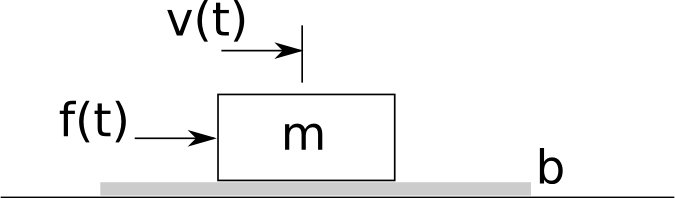
\includegraphics[width=\FigWidth\textwidth]{mass_damper.png}
\caption{Sketch of a simplified automobile model.  The point mass ($m$) moves to the right at a velocity ($v(t)$.  The input is a force ($f(t)$) and the drag force ($b (v(t))$ resists the motion. }
\label{f:massd}
\end{figure}
Based on this sketch we can do things like draw a free-body-diagram and apply Newtonian principles to arrive at an equation of motion.  We might also make an ambitious simplifying assumption that the drag force that resists the motion of the mass is linearly related to the velocity, i.e., $f_{\mathrm{drag}}=b(v(t))$.  Then we could come up with an equation of motion
\begin{equation}
\label{e:car}
m\left(\dot{v}(t)\right) + b(v(t)) = f(t)
\end{equation}
where $m$ is the mass of the car, $v(t)$ is the speed, $\dot{v}(t)$ is the acceleration, $b$ is the coefficient of linear drag and $f(t)$ is the input force.  This equation of motion is our mathematical model
This equation has the same form (a first-order, linear, ordinary differential equation) as our first-order model~(\ref{e:first}).

This is meant to be an example of a model that is obviously wrong.  A physical automobile is a complex system with many, many degrees of freedom.  Our simplified model~(\ref{e:car}) is meant to do just one thing, allow us to predict how, in general, the speed of a car responds to changes in the throttle input.


\section{Step Response}\label{s:firststep}
One useful aspect of our first-order model~(\ref{e:first}) is that the solution to this differential equation is well known for a variety of input functions.  A particularly interesting input function is the \gls{step function} ($\mu(t)$) defined as
\begin{equation}
\label{e:step}
\mu(t)= \left\{ 
\begin{array}{cl}
0 & \, \mathrm{for}\, t < 0 \,\,\,\\
1 & \, \mathrm{for}\, t \geq 0
\end{array} \right.
.
\end{equation}
This function ($\mu(t)$) is also known as the \emph{unit} step function because the amplitude of the step is 1.0.
Figure~\ref{f:step} illustrates how the value of $\mu(t)$ is zero before $t=0$ and then instantaneously changes to unity.
\begin{figure}[hbt!]
\centering
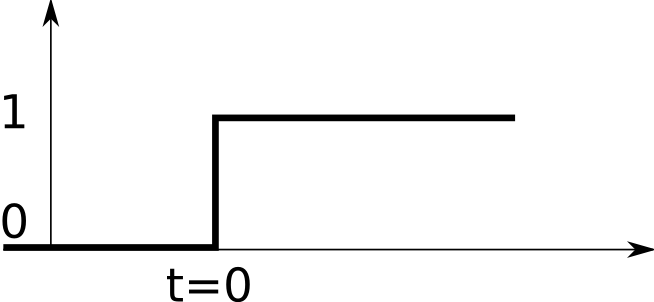
\includegraphics[width=\FigWidth\textwidth]{step.png}
\caption{Illustration of a step function $\mu(t)$.}
\label{f:step}
\end{figure}

Now consider our generic first-order model (\ref{e:first}) with a step input ($f(t)=A\mu(t)$) and an initial condition of zero ($y(0)=0$),
\begin{equation}
\label{e:firststepinput}
\frac{dy(t)}{dt} + \frac{1}{\tau}y(t) = A\mu(t).
\end{equation}
(You should notice that the input function ($f(t)$) is a step input with an amplitude of $A$.)
The \gls{step response} is the solution to this ordinary differential equation which is
\begin{equation}\label{e:stepresp}
y(t) = A\tau\left(1-e^{-t/\tau}\right)
\end{equation}
for $t>0$.  Notice that there are two key parameters of our model step response: the time constant ($\tau$) and the amplitude of the step input ($A$).

\begin{figure}[hbt]
\centering
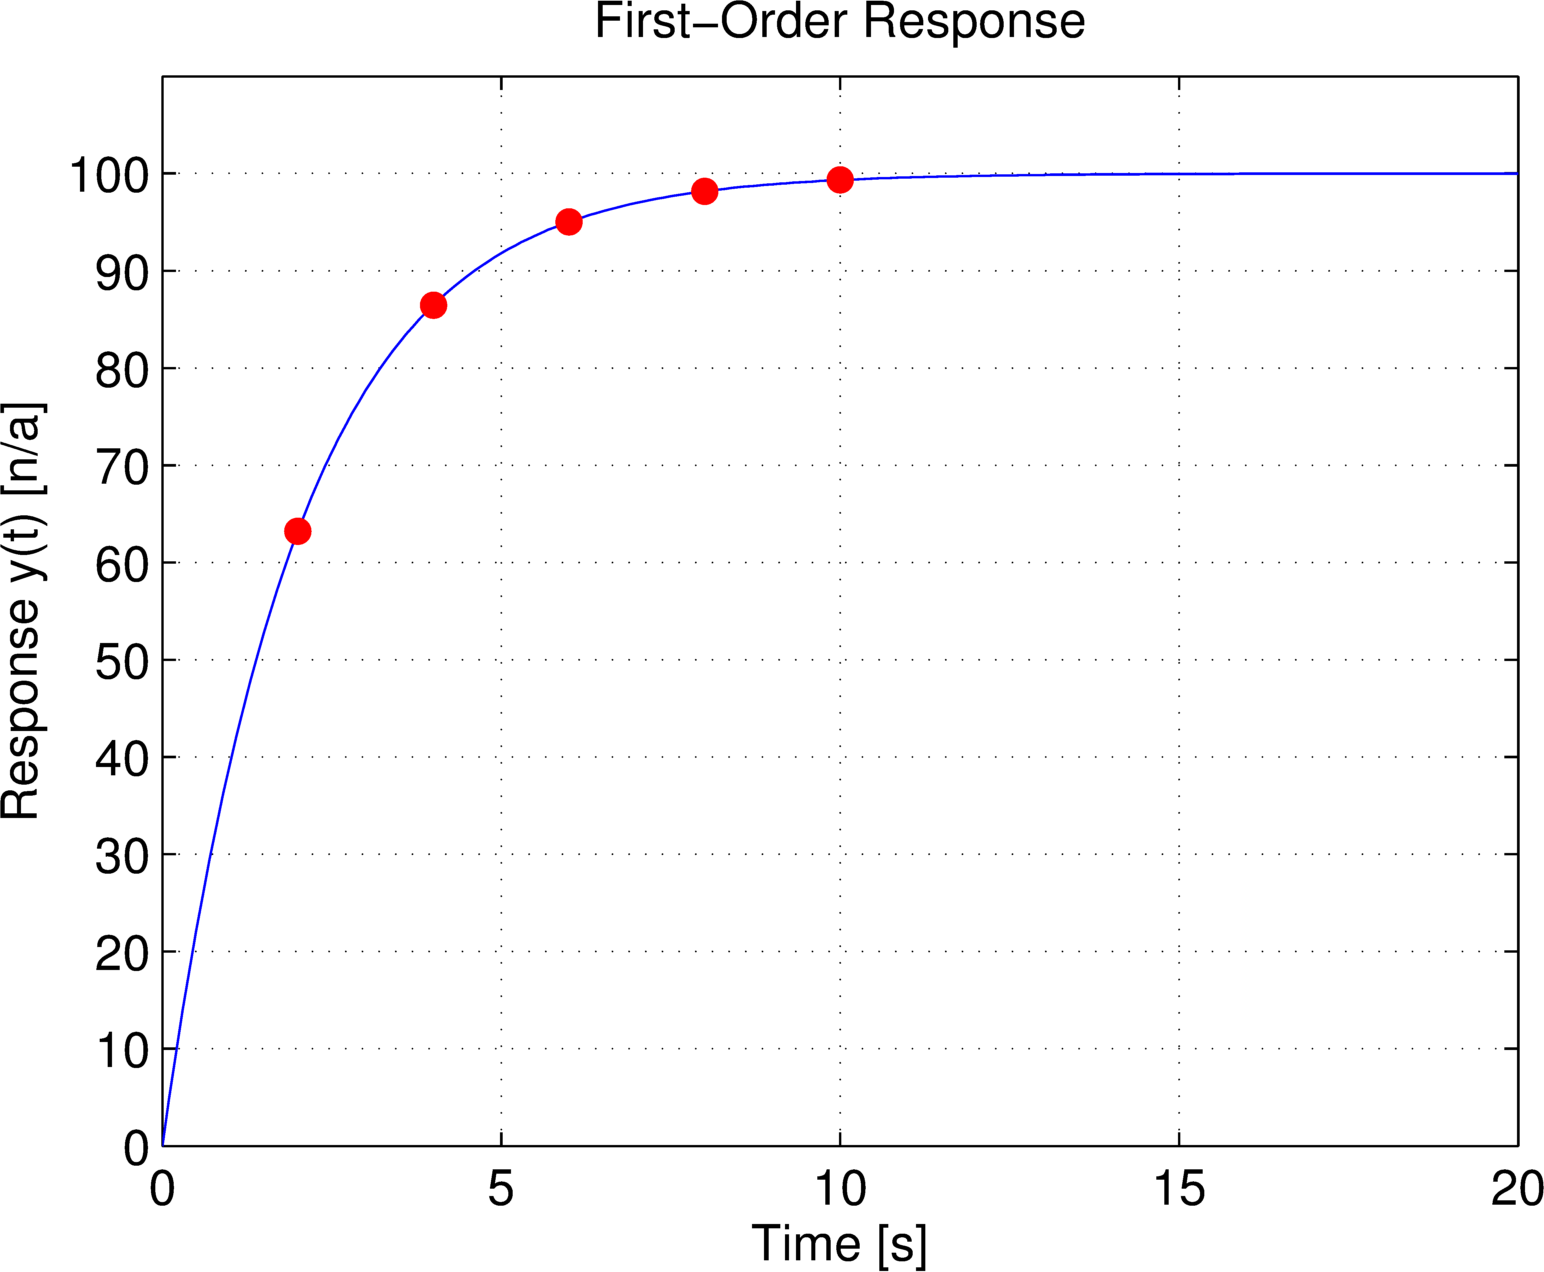
\includegraphics[width=\textwidth]{first_step.png}
\caption{Graph of the step response (\ref{e:stepresp}) with $\tau=\unit[2]{s}$ and $A=50$.  The red dot markers indicate the value of the solution at $t=[\tau,2\tau,3\tau,4\tau,5\tau]$. }
\label{f:firststep}
\end{figure}


\lstinputlisting[style=myMatStyle,
caption={Script for first-order response: first\_order\_response.m},
label={l:firstresp}]
{../code/first_order_response.m}


This solution (\ref{e:stepresp} is graphed in Figure~\ref{f:firststep} using the MATLAB script in Listing~\ref{l:firstresp}. This time response to a step input (or step response for short) has a characteristic shape as it rises and approaches the \gls{steady-state response} exponentially.  One important aspect of the response is that it approaches a new constant value, the steady-state response.  A simple way to find the steady state value is to set $\dot{y}(t)=0$ in (\ref{e:first}).  Since we are looking for the ``steady-state'' value we can anticipate that all rates of change (derivatives) will be zero.  Now the steady-state value ($y_{\mathrm{ss}}$) is 
\begin{equation}\label{e:ss}
y_{\mathrm{ss}} = \tau A.
\end{equation}

Another important characteristic of this model is that the response ($y(t)$) moves exponentially from the initial value to the steady state value.  This response is characterized by the the \gls{time constant} ($\tau$).  If we evaluate time response (\ref{e:stepresp}) at $t=\tau$ we find that
\[
y(t=\tau) = A \tau (0.632) = 0.632 (y_{\mathrm{ss}})
\]
which means that after one time constant has passed the response is 63.2\% of the way from the initial value to the steady state value.  Take a look at Figure~\ref{f:firststep} to make sure that we did the math correctly!

\subsection{Car Example---Step Response}
Now that we've discussed the time response of our first-order model let's see how this applies to our automobile model.  We can rearrange the mathematical model (\ref{e:car}) so that it looks more like our generic model (\ref{e:first}) which results in the expression
\begin{equation}\label{e:car2}
\dot{v}(t) + \frac{1}{m/b}(v(t)) = \frac{F}{m}\mu(t)
\end{equation}
which highlights that the time constant is $\tau=m/b$ and that the steady state speed is $v_{\mathrm{ss}}=F/b$.  Take a moment to think about this.  It means that the larger the mass of our car, the slower the acceleration (because the time constant is larger).  You might also notice that the mass has no effect on the steady state speed; our model says that a heavy ``car'' will reach the same final speed as a light car, it will just get there slower.  Finally we might notice that the more drag in our model, the slower our ``car'' will go for the same input. Listing~\ref{l:carresp} illustrates how we might use MATLAB to graph the solution for specific numerical values.

\lstinputlisting[style=myMatStyle,
caption={Script for first-order response of our car example: firstorder\_car\_ex.m},
label={l:carresp}]
{../code/firstorder_car_ex.m}

\begin{ex}
The step function in (\ref{e:step}) could be more precisely called the ``unit step function'' because it has an amplitude of 1.  Write an equation (similar to (\ref{e:step})) and sketch a graph (similar to Figure~\ref{f:step}) for the more general step function input $f(t) = A(\mu(t-t_o))$.
\end{ex}

\begin{ex}
We justified (\ref{e:ss}) by starting with the model (\ref{e:first}).  Another way to calculate the steady state response is to evaluate the solution (\ref{e:stepresp}) as $t \to \infty$.  Show that using this method yields the same result.
\end{ex}

\begin{ex}
We showed that the response of a first-order model to a step function input has an exponential increase characterized by the time constant.  Furthermore we showed that after a duration of one time constant beyond the rise in the step input the output will be 63.2\% of the way to its steady state value.  Figure~\ref{f:firststep} illustrates the value of the response at  $t=[\tau,2\tau,3\tau,4\tau,5\tau]$.  Evaluate \ref{e:stepresp} for these values of time and report the results in a two column table where the first column is the ratio $t/\tau$ and the second column is the ratio $y(t)/y_{\mathrm{ss}}$.
\end{ex}

\begin{ex}
\label{ex:carstep}
Consider the step response to our car model (\ref{e:car2}) with the following parameters: mass = \unit[800]{kg}, drag coefficient = \unitfrac[225]{Ns}{m}, step input amplitude = \unit[15,000]{N}.  Using MATLAB, create a graph similar to Figure~\ref{f:firststep} to illustrate the step response of our ``car''.  Annotate the graph to show the time constant and the steady state speed.  Also, make sure to use appropriate units for each axis.
\end{ex}

\begin{ex}
Consider the step response to our car model (\ref{e:car2}) with the parameters given in Exercise~\ref{ex:carstep}
\begin{itemize}
\item What is the minimum step input amplitude ($F_{\mathrm{min}}$) that would cause our ``car'' to go from \unit[0--60]{mph}?
\item Based on this minimum step input amplitude, how long does it take for the ``car'' to go from \unit[0--60]{mph}? (Hint: the answer to this question can be a number or a sentence!)
\item If we double $F_{\mathrm{min}}$
 \begin{itemize}
 \item How long does it take for the ``car'' to go from \unit[0--60]{mph}?
 \item What is the new top speed (in mph)?
 \item How long does it take for the ``car'' to achieve this new top speed?
 \end{itemize}
\end{itemize}
\end{ex}

\ifsolutions
\begin{soln}
Here is a solution.
\begin{itemize}
\item The steady-state value is $V_{ss}=F/b$ and \unit[60]{mph} is approximately \unitfrac[27]{m}{s}.  Since $b=\unitfrac[225]{Ns}{m}$, $F_{min}=\unit[6075]{N}$.
\item Interestingly the car never truly gets all the way to the final steady-state value!  After five time constants ($t=5\tau$=\unit[25]{s}) the car is 99\% of the way to \unit[60]{mph}
\item If we double this input force...
\begin{itemize}
\item The car takes about \unit[4]{s} to get to \unit{60}{mph} (\unitfrac[27]{m}{s}).
\item The new top speed is double of the original top speed---\unit[120]{mph}.  This is because the system is linear!
\item Again, it never really gets there.  It gets 99\% of the way there after five time constants: $\tau=m/b=\unit[3.5]{s}$ so $5\tau=\unit[17.8]{s}$.
\end{itemize}
\end{itemize}
\end{soln}
\fi


\section{Free Response}
Another useful time response of our first-order model is the response with no input ($f(t)=0$) and an initial condition ($y(0)=y_o$).  The solution to (\ref{e:first}) under these conditions is 
\begin{equation}\label{e:firstfree}
y(t) = y_o \, e^{-t/\tau}
\end{equation}
for $t>0$. Figure~\ref{f:firstfree} illustrates this free response.  Just as before the time constant is the key factor that determines the characteristic of the response.  Again, at $t=\tau$ the output has fallen by 63.2\%.
\begin{figure}[hbt]
\centering
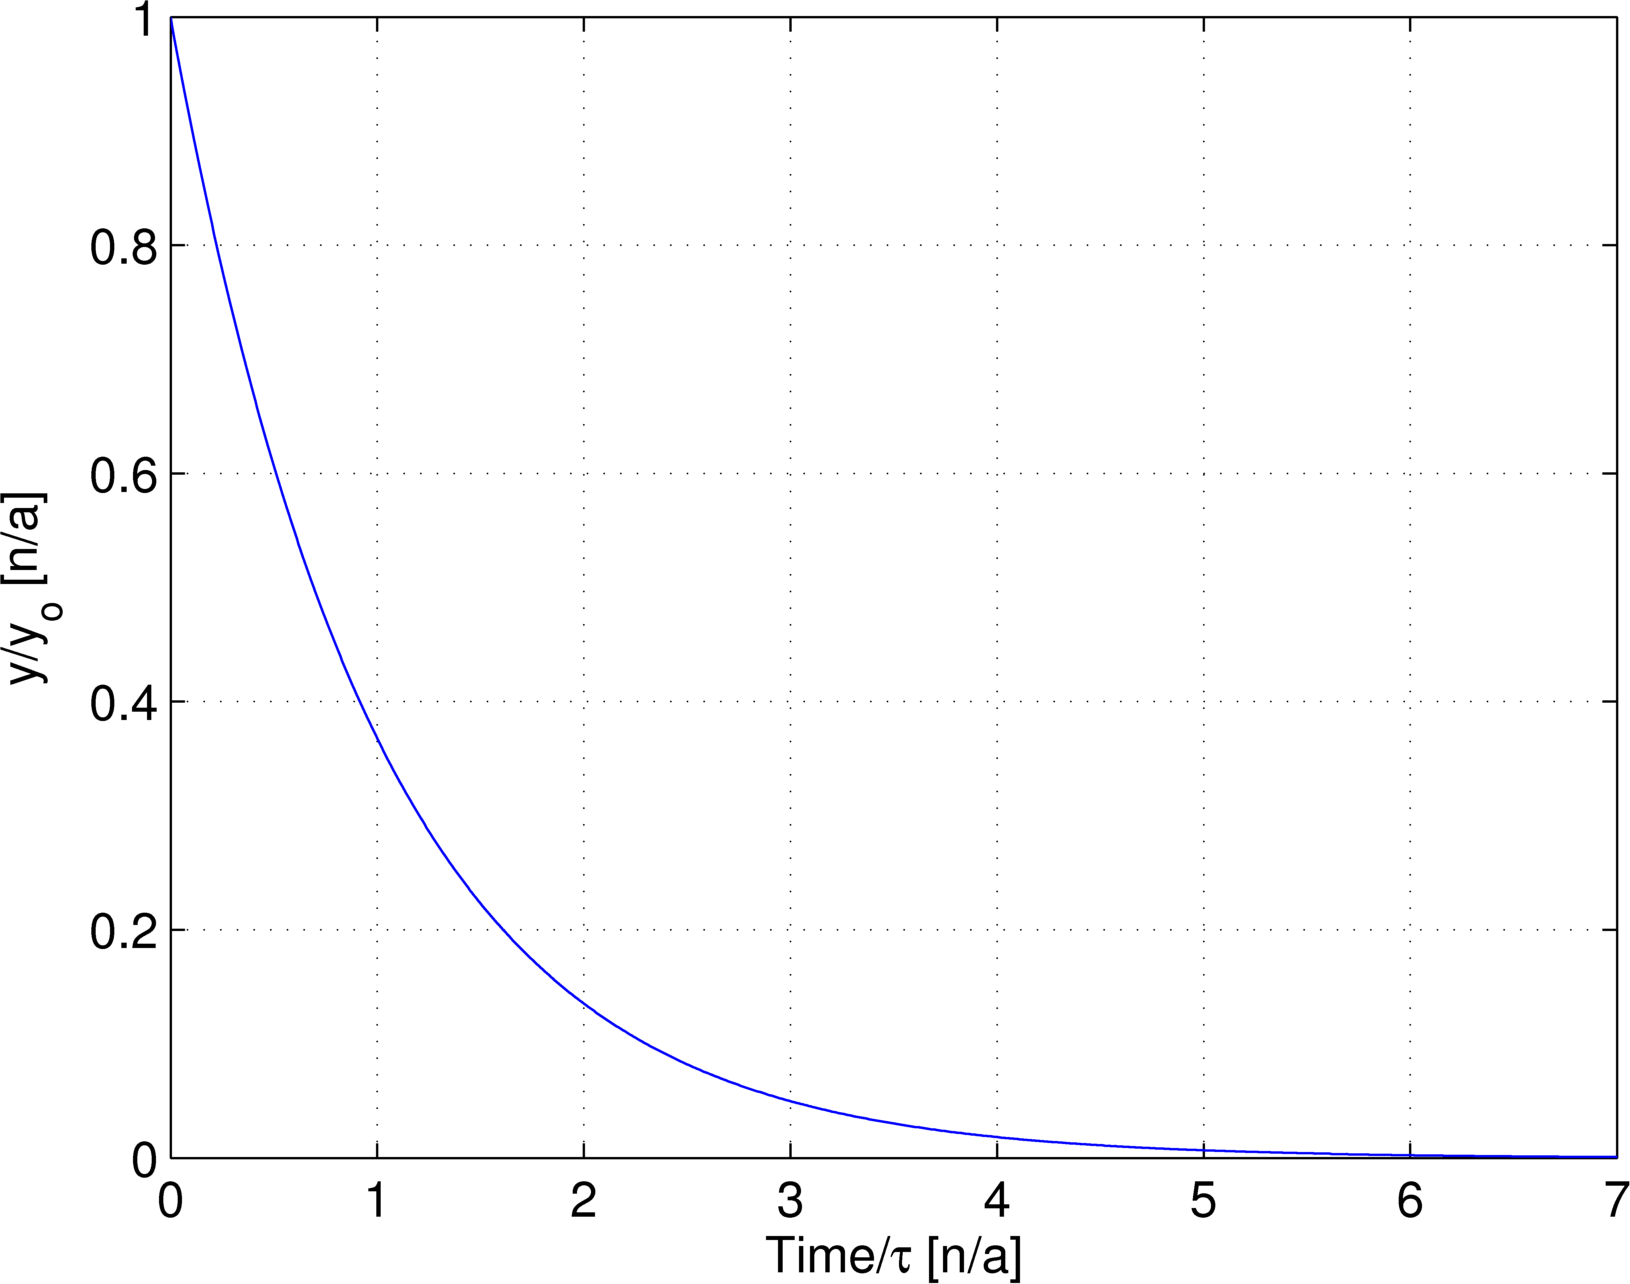
\includegraphics[width=\FigWidth\textwidth]{firstfree.png}
\caption{Graph of the free response (\ref{e:firstfree}).  Notice that the $x$ and $y$ axes have been normalized so that the output is the ratio of the response and the initial condition and the time is the ratio of time and the time constant.}
\label{f:firstfree}
\end{figure}

\begin{ex}
Using our automobile model (\ref{e:car}), write an expression for the free response of this model with appropriate physical parameters.  Create a graph of the free response with the initial condition $v(0)=\unit[60]{mph}$. For the x-axis of the graph use the units mph and for the y-axis of the graph use the units seconds.
\end{ex}



\section{Superposition---Step Response with Non-Zero Initial Condition}
One the characteristics that make linear system such as our first-order model useful is the principle of \gls{superposition} which allows determine the solution to a linear model by adding together multiple solutions.  As an example, suppose there are two input functions, $f_1(t)$ and $f_2(t)$, and that the corresponding solutions are $y_1(t)$ and $y_2(t)$.  If we want to know the response of the system to both inputs, $f(t)=f_1(t)+f_2(t)$, we can simply add the two solutions, $y(t)=y_1(t)+y_2(t)$. 

This principle simplifies the task of finding the response to our first-order model when there are both initial conditions and a forcing function.  Armed with superposition principle we can determine the step response (the solution to (\ref{e:first}) with the input $f(t)=A\mu(t)$) of our first-order model when there is a non-zero initial condition ($y(0)=y_o$) by simply adding our two previous solutions, the step response with zero initial condition and the free response with no forcing function:
\begin{equation}
y(t) = y_o \, e^{-t/\tau} + A\tau\left(1-e^{-t/\tau}\right).
\end{equation}

Another handy aspect of superposition is the scaling property.  This means that if we scale (multiply) the input by a factor ($a$) then the output is simply the response to the original input scaled (multiplied) by the same factor.  As an example, consider our first-order car model (\ref{e:car}) where the input is a force ($f(t)$).  If we know that a force of \unit[1,000]{N} results in a steady state speed of \unit[25]{mph} then superposition tells us that a force of \unit[2,000]{N} will result in a final speed of \unit[50]{mph}.

\begin{ex}
Consider our first-order car model discussed above where a \unit[1,000]{N} input yields a steady state speed of \unit[25]{mph}.  Furthermore, we know that the time constant of this system is \unit[2]{s}.  Again we double the input to from \unit[1,000]{N} to  \unit[2,000]{N}. What is the time constant of the response with the doubled input?

Hint: This might be considered a 'trick' question.
\end{ex}



%\section{Second-Order Model}

\section{Second-Order Model}
We will use \gls{second-order model} as shorthand for a linear, ordinary, time-invariant second-order differential equation of the form
\begin{equation} \label{e:second}
\ddot{y}(t) + 2 \zeta \omega_n \dot{y}(t) + \omega_n^2 y(t) = f(t)
\end{equation} 
where 
\begin{itemize}
\item $\ddot{y}(t)$ is the second derivative of $y(t)$ with respect to time,
\item $\dot{y}(t)$ is the first derivative of $y(t)$ with respect to time,
\item $y(t)$ is the solution to (\ref{e:second}),
\item $\zeta$ is the \gls{damping ratio},
\item $\omega_n$ is the \gls{undamped natural frequency} and
\item $f(t)$ is the input, or forcing function.
\end{itemize}
Just as with our first-order and static (zero-order) models, this model is an abstraction; it never has exactly the same behavior of a physical system, but it has been proven to be a useful approximation for the behavior of a variety of phenomena.  To understand the model we'll first present the solution to (\ref{e:second}) for a few types of input (forcing functions) and then work through some examples of cases where the model is a helpful abstraction of physical systems.

The intent of the following discussion is meant to be a summary and/or review of what you have seen in other courses (Differential Equations, System Dynamics, Feedback Controls, etc.).  The discussion should be sufficient for our purposes of modeling and measurement, but it is by no means an exhaustive treatment of analysis of second-order models or harmonic oscillator models.

Also, for now we are only interested in {\bf underdamped} and {\bf undamped} versions of the model (\ref{e:second}) where $0 \leq \zeta < 1.0$.  Another way to say this is that we are only interested in second-order models that have oscillations in their response.

\subsection{Example: Mass-Spring-Damper}
One type of physical system that has similar behavior to our second-order model is the mass-spring-damper system illustrated in Figure~\ref{f:msd2}.  (Actually, this system is still a bit of an abstraction; we rarely encounter applications that require a point mass attached to a mass-less spring.  The abstraction is meant to represent any physical system where there is inertia (mass, kinetic energy), a restoring force (spring, potential energy) and motion resistance (damper, energy dissipation).)
\begin{figure}[htb!]
\centerline{
{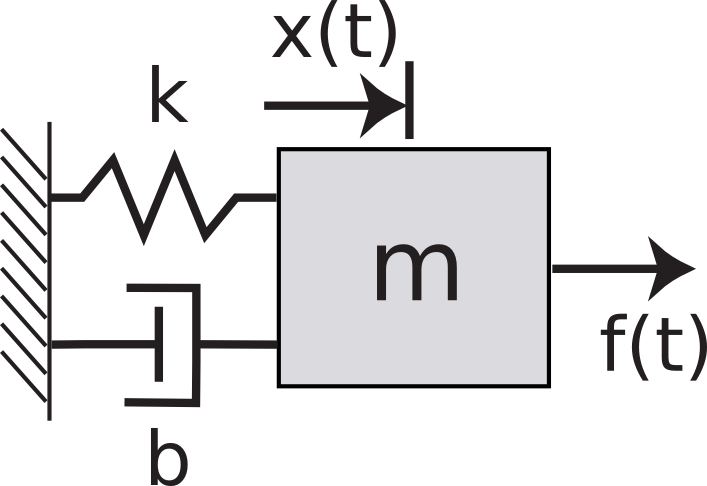
\includegraphics[width=0.4\textwidth]{msd_lower.png}}}
\caption{Sketch of a mass-spring-damper system.}
\label{f:msd2}
\end{figure}

If you draw a free-body-diagram of this system, you should be able to derive the second-order equation of motion
\begin{equation}\label{e:msd}
m \ddot{x}(t) + b \dot{x}(t) + k x(t) = f(t)
\end{equation}
where $m$ is the mass, $b$ is the linear damping coefficient, $k$ is the linear spring constant, $x(t)$ is the displacement of the mass and $f(t)$ is the input force.

\begin{ex}
Using (\ref{e:second}) and (\ref{e:msd}), derive expressions for the system parameters ($\omega_n$ and $\zeta$) in terms of the physical parameters ($m$, $b$, and $k$).  (Hint: Use physical units to check your answers.)
\end{ex}

\ifsolutions
\begin{soln}
You should verify that the following expressions are correct:
\[ \omega_n = \sqrt{k/m} \; \; \; \unitfrac[]{rad}{s}\]
\[ \zeta = \frac{b}{2 \sqrt{mk}} \; \; \; \unitfrac[]{n}{a} \]
\end{soln}
\fi


\section{Free Response}\label{s:secondfree}
The free response for our model is the solution to the second-order model (\ref{e:second}) with initial conditions, but no forcing function (also known as the homogeneous equation)
\begin{equation} \label{e:secondhomo}
\ddot{y}(t) + 2 \zeta \omega_n \dot{y}(t) + \omega_n^2 y(t) = 0
\end{equation} 
where the initial conditions at $t=0$ are
\begin{itemize}
\item $y(0) = y_o$ and 
\item $\dot{y}(0)=\dot{y}_o$.
\end{itemize}
Hopefully you've been convinced that this type of differential equation is straightforward to solve (in theory), and we can present (without derivation) that the solution to this equation is the function
\begin{equation} \label{e:secondfree}
y(t) = C \left(e^{-\zeta \omega_n t}\right) \left( \cos(\omega_d t - \phi) \right).
\end{equation}
where
\begin{eqnarray}\
\omega_d & = & \omega_n \sqrt{1-\zeta^2}, \label{e:damped} \\
C & = & \sqrt{ y_o^2 + \left( \frac{\dot{y}_o+\zeta\omega_n y_o}{\omega_d} \right)^2 } \;\;\;\;\;\;\;\;\; \mathrm{and}\label{e:C} \\
\tan(\phi) & = & \frac{\dot{y}_o+\zeta \omega_n y_o}{\omega_d y_o}. \label{e:phi}
\end{eqnarray}

The free response (\ref{e:secondfree}) is the key part of all this.  There are many systems that behave in this general way with a decaying oscillatory response.  To illustrate this we can annotate the equation to highlight the three parts of the solution:
\begin{equation} \label{e:secondfree_annote}
y(t) = \underbrace{C}_\text{constant} 
\underbrace{\left(e^{-\zeta \omega_n t}\right)}_\text{exponential decay}
\underbrace{\left( \cos(\omega_d t - \phi) \right)}_\text{oscillation}.
\end{equation}
One important detail is that there are two slightly different ``natural frequencies'' to keep track of.  The \gls{undamped natural frequency} ($\omega_n$) is the parameter we saw in the system model and which is included in the exponential decay component of (\ref{e:secondfree_annote}).  The \gls{damped natural frequency} ($\omega_d$) is the frequency of oscillation, the angular frequency inside the $\cos$ term of (\ref{e:secondfree_annote}).  The relation between the two values is given in (\ref{e:damped}).  For small values of $\zeta$, so called ``lightly damped systems'', there is little difference between the two values.

Another way to ``see'' this solution is to graph the time response.  The short MATLAB script in Listing~\ref{l:secondfree} generates Figure~\ref{f:secondfree}.  This figure illustrates the key characteristics of a second order free response:
\begin{enumerate}
\item the system oscillates at a constant frequency (the $\cos(\omega_d t)$ term) and
\item the amplitude of the oscillations decays exponentially over time (the $e^{=\zeta \omega_n t}$ term).
\end{enumerate}
%\lstinputlisting[style=myMatStyle,
%caption={Script for plotting the free response of a second-order model (\verb+second_order_free.m+).},
%label={l:second_free}]
%{./code/second_order_free.m}

\lstinputlisting[style=myMatStyle,
caption={Script for plotting the free response of a second-order model. (Filename=second\_order\_free.m, \url{http://web.eng.hawaii.edu/~bsb/me402/book/code/second_order_free.m})},
label={l:secondfree}]
{../code/second_order_free.m}


\begin{figure}[hbt]
\centering
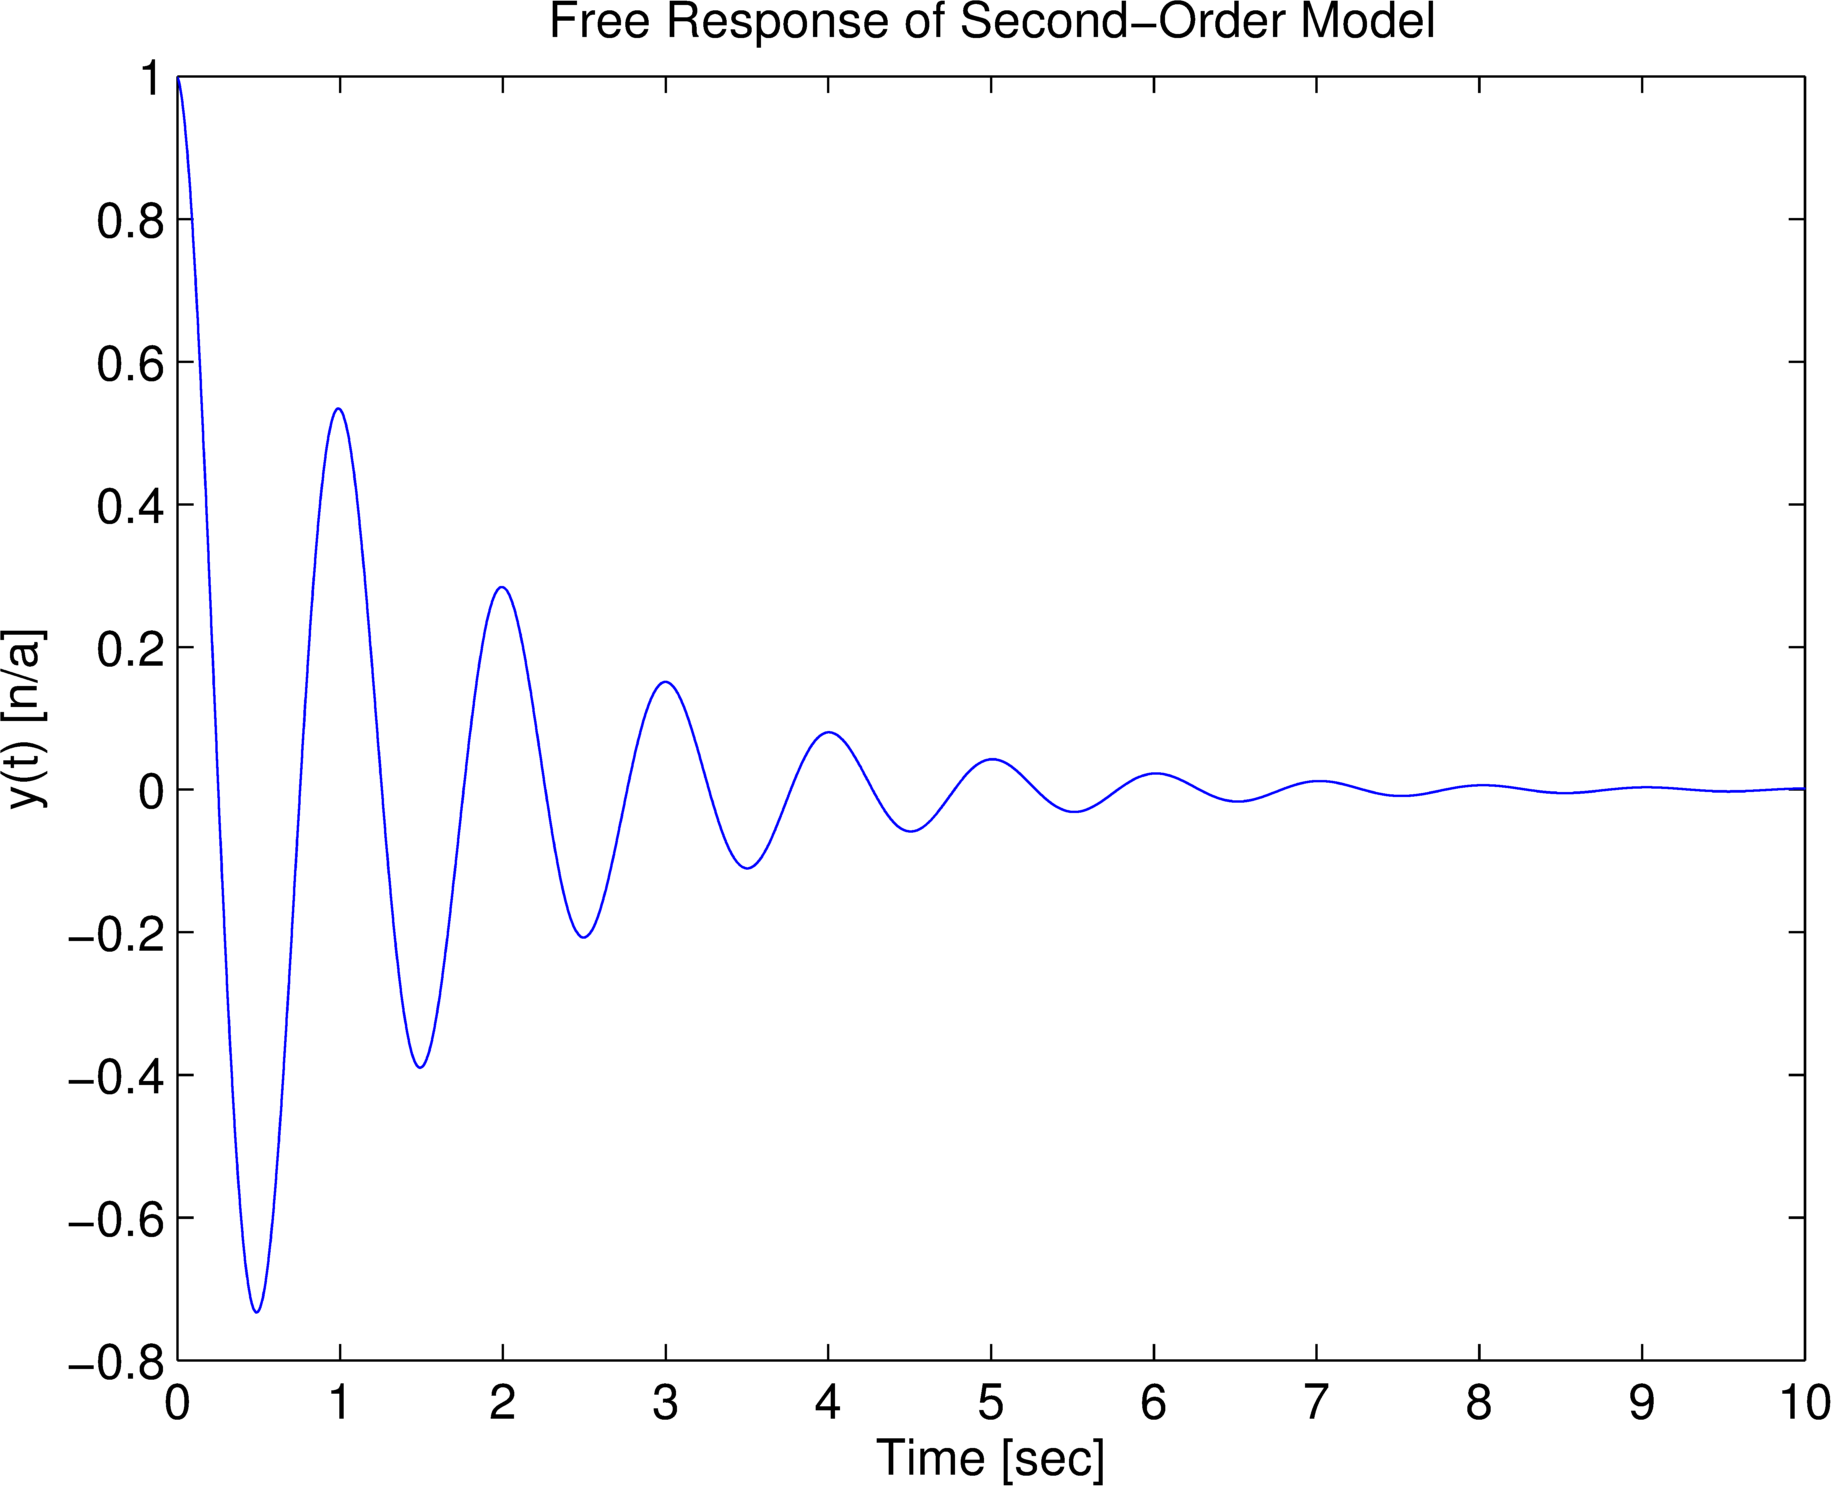
\includegraphics[width=\FigWidth\textwidth]{second_free.png}
\caption{Graph of the free response (\ref{e:stepresp}) with $\omega_n= \unit[1]{Hz}$, $\zeta=0.1$ (10\%) and $y(t=0)=1$.}
\label{f:secondfree}
\end{figure}

\begin{ex}
There is a mistake in Listing~\ref{l:secondfree} which attempted to display the solution for the case where there is only a ``displacement'' initial condition: i.e., $y(0)=y_o$ and $\dot{y}(0)=0$.  The mistake is that the solution in the code uses the values $C=y_o$ and $\phi=0$ which are not correct (but they are close). 
\begin{itemize}\label{ex:secondresp}
\item Derive expressions for the constants $C$ and $\phi$ based on the initial conditions $y(0)=y_o$ and $\dot{y}(0)=0$.
\item Copy the script in Listing~\ref{l:secondfree} and create the graph shown in Figure~\ref{f:secondfree}.
\item Correct the script in Listing~\ref{l:secondfree} and plot a second curve, on the same axes, with the corrected solution for $y_o=1$.  
  \begin{itemize}
  \item Include your MATLAB script with your solution.
  \item Include your graph as a properly formatted figure.
  \end{itemize}
\end{itemize}
The error is simply in the calculation of $C$ and $\phi$; the structure of the script in Listing~\ref{l:secondfree} should work just fine.
\end{ex}

\ifsolutions
\begin{soln}
\[ C = \sqrt{\frac{y_o}{1-\zeta^2}} \]
\[ \tan\phi = \frac{\zeta}{\sqrt{1-\zeta^2}} \]
or 
\[ \phi = \arctan\left(\frac{\zeta}{\sqrt{1-\zeta^2}}\right) \]

See Figure~\ref{f:secondfreesoln}.  This figure is generated using Listing~\ref{l:seconfree2}

\lstinputlisting[style=myMatStyle,
caption={Script for plotting the corrected free response of a second-order model.},
label={l:secondfree2}]
{../code/soln/second_order_free_correct.m}

\begin{figure}[hbt]
\centering
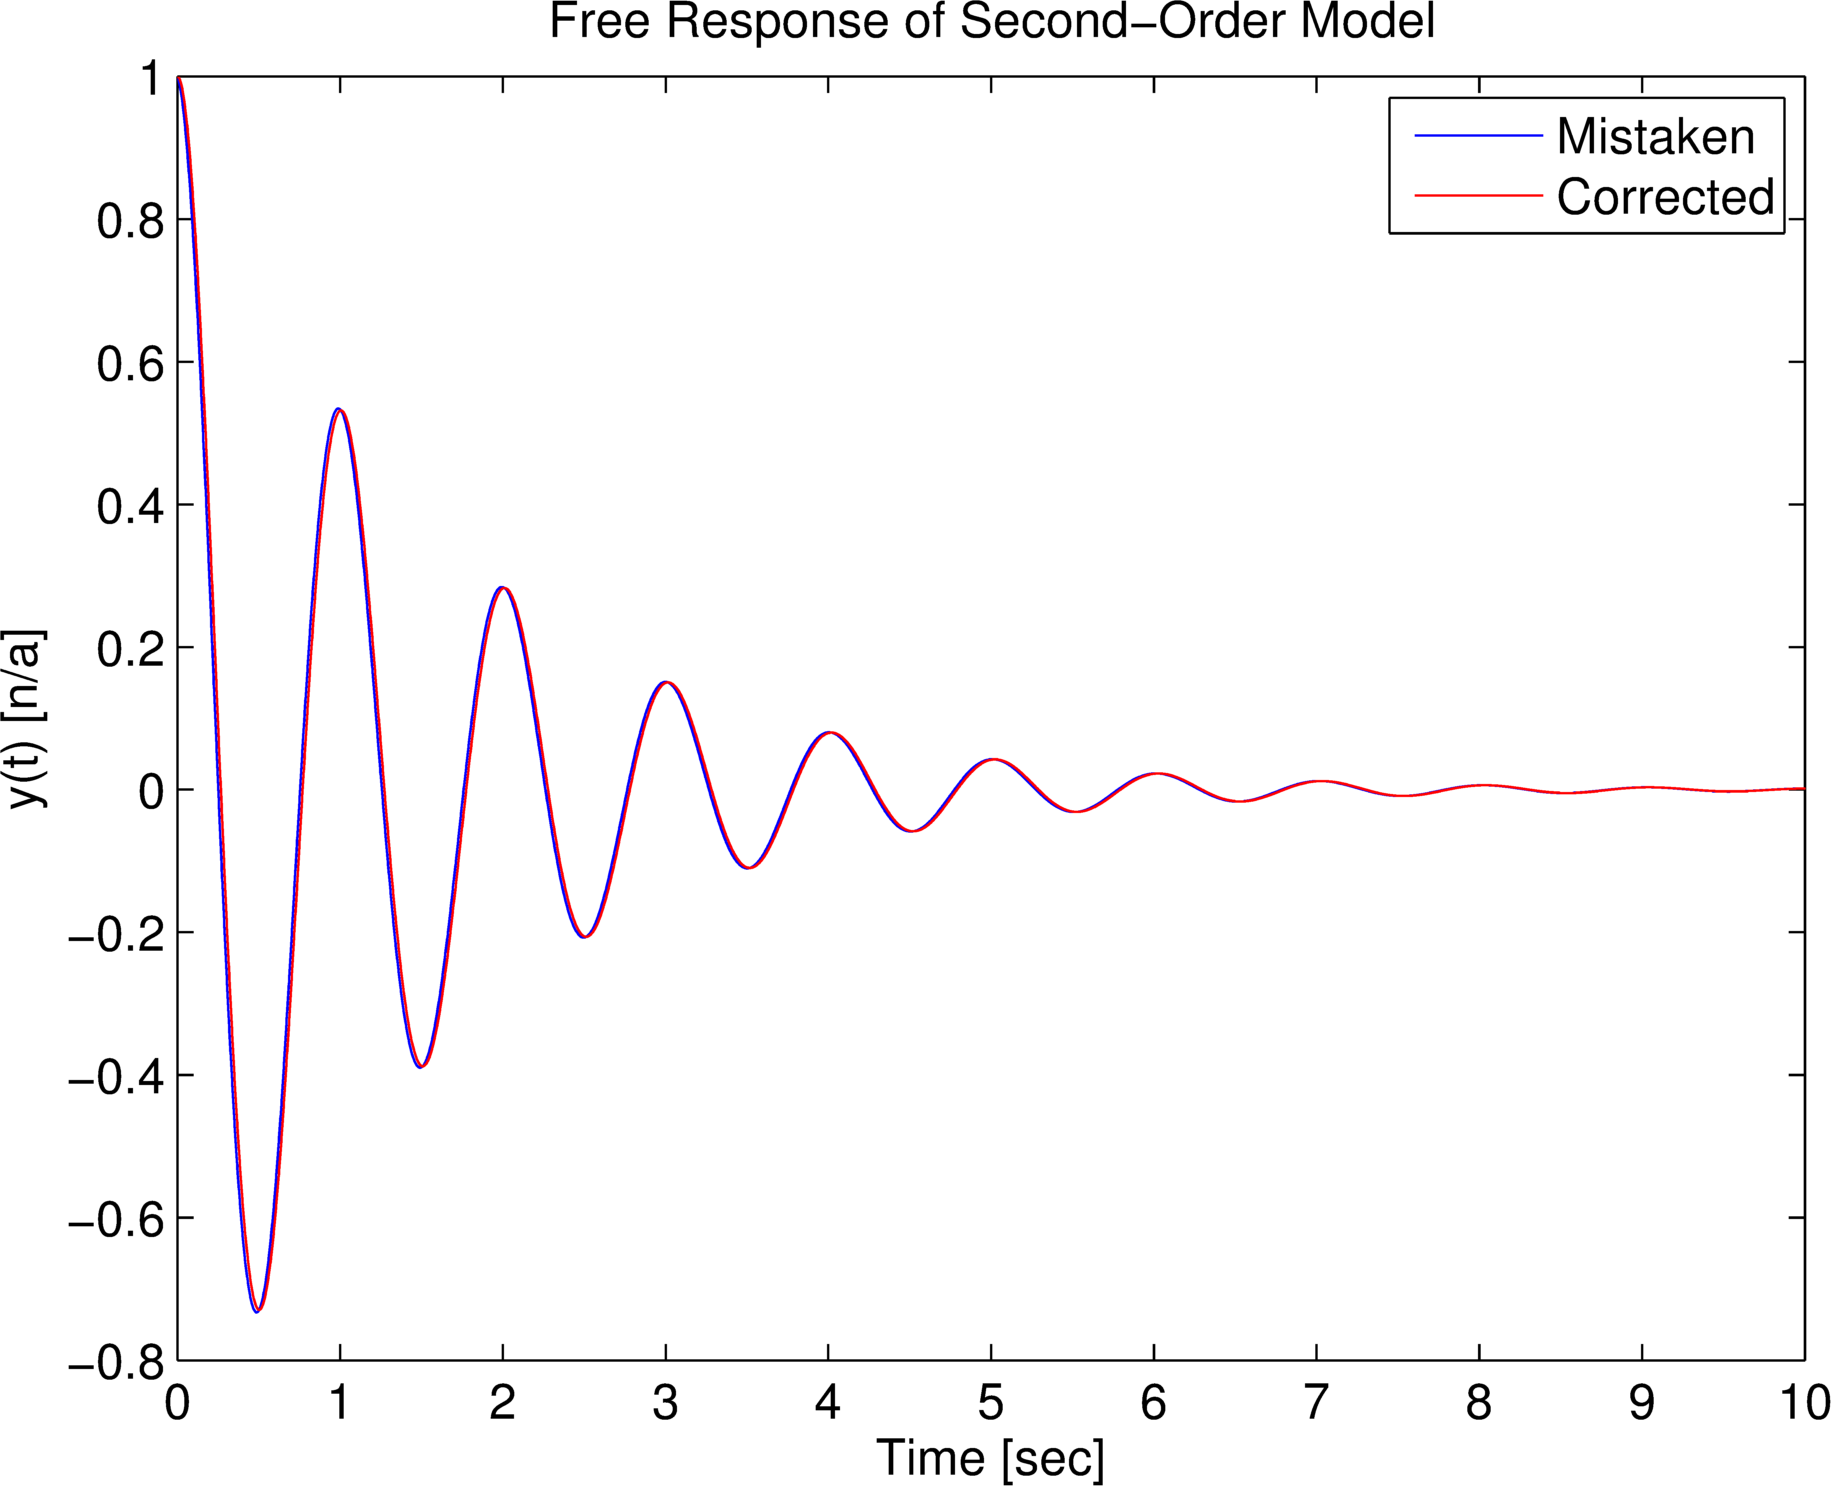
\includegraphics[width=\FigWidth\textwidth]{second_free_soln.png}
\caption{Graphs of the original mistaken free response and the corrected free response.}
\label{f:secondfreesoln}
\end{figure}
\end{soln}
\fi

\begin{ex}
Consider the effect of the damping ratio ($\zeta$) on the shape of free response.  Using Listing~\ref{l:secondfree} as a starting point, use MATLAB to create a single graph for the free response with the initial conditions $y(0)=1$ and $\dot{y}(0)=0$.  On a single set of axes, plot the response for systems with the following values for the damping ratio: $\zeta=\{0.0, 0.01 , 0.1, 0.5, 0.9\}$.  Use a legend to declare which curve is associated with each value of $\zeta$.  Submit this single graph as an appropriately formatted figure with a short description of what you observe about the effect of changing $\zeta$.
\end{ex}

\ifsolutions
\begin{soln}
See Figure~\ref{f:secondfreezetas} generated using Listing~\ref{l:secondfreezeta}.

\lstinputlisting[style=myMatStyle,
caption={Script for plotting the free response of a second-order model with varios values of zeta.},
label={l:secondfreezeta}]
{../code/second_order_free_zeta.m}


\begin{figure}[hbt]
\centering
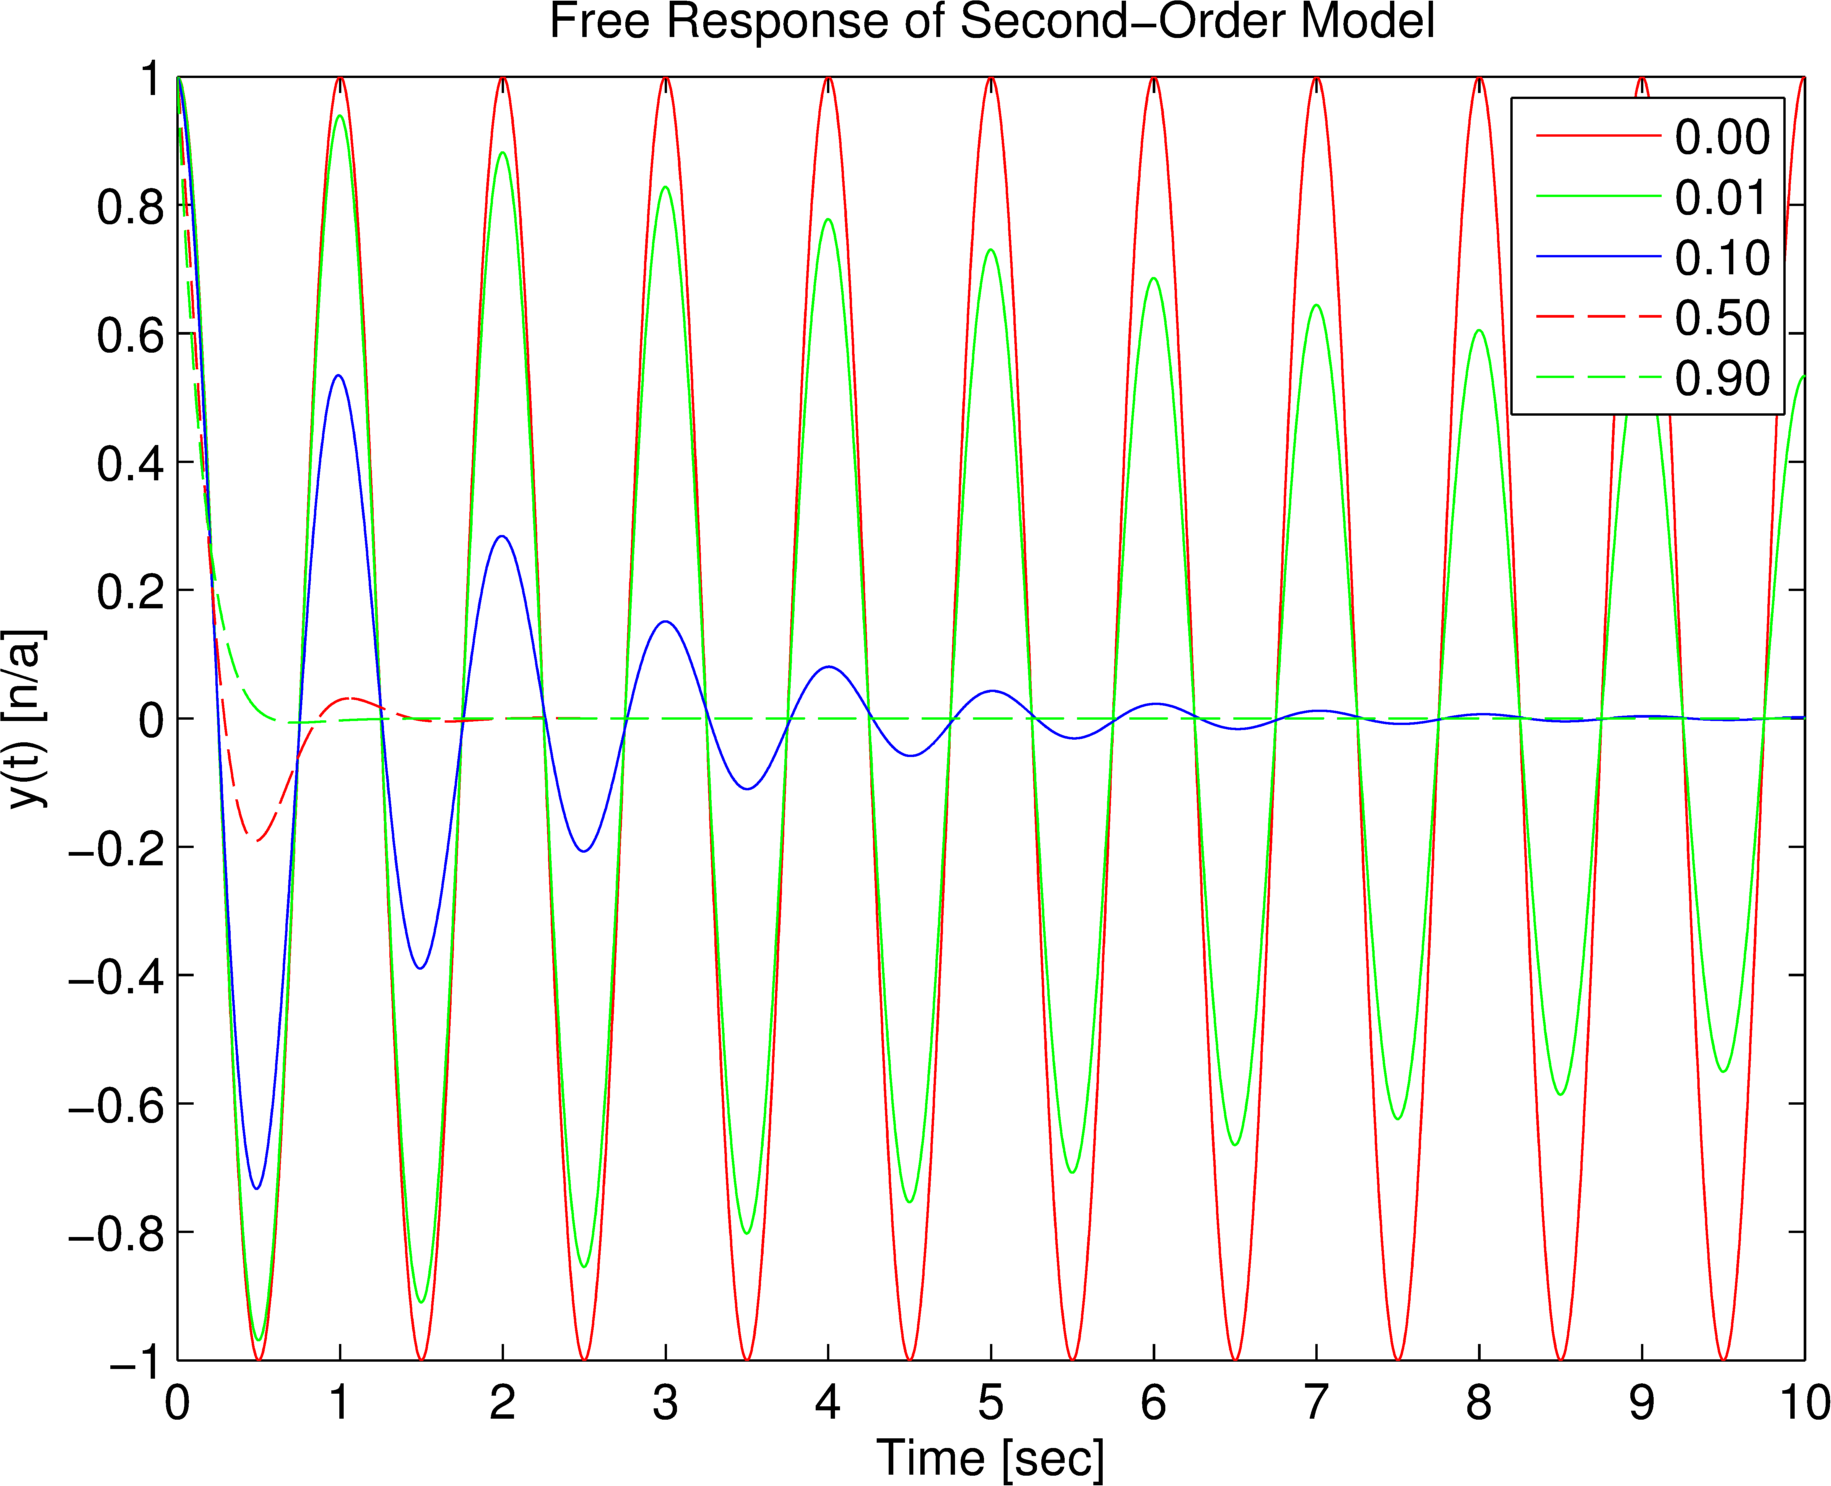
\includegraphics[width=\FigWidth\textwidth]{free_zetas.png}
\caption{}
\label{f:secondfreezetas}
\end{figure}

\end{soln}
\fi

\begin{ex}
Consider the model's free response to velocity-only initial conditions---$y(0)=0$ and $\dot{y}(0)=v_o$.
\begin{itemize}
\item Derive expressions for the constants $C$ and $\phi$ based on these initial conditions.
\item Substitute your expressions into the response (\ref{e:secondfree}) and write a simplified equation for the response.  (Hint: $\cos\left(u-\frac{\pi}{2}\right) = \sin(u)$.)
\item Using MATLAB, create a figure the graphs the response ($y(t)$) to this initial condition.
\end{itemize}
\end{ex}


\begin{ex}
Given a damping ratio of $\zeta=0.01$ (1\% damping), write and expression for the damped natural frequency as a function of the undamped natural frequency.  \\
Repeat the exercise for a 10\% damping.
\end{ex}



%\section{Example: Cantilevered Beam}

\section{Example: Cantilevered Beam}
Another physical system that has a response that can be approximated by our second-order model is a cantilevered beam.  Imagine a yardstick fixed on one end.  When the free end is subject to a displacement (the initial condition) and then released, the tip will oscillate.  A cantilevered beam, unlike our lumped mass system in Figure~\ref{f:msd2}, is a continuous system, but for now we'll approximate it by examining the first natural frequency.  

\subsection{First-Mode of Cantilevered Beam}
The first natural frequency of a uniform cantilevered beam, Figure~\ref{f:blevins}, can be estimated by using classical beam theory.
\begin{figure}[htb!]
\centerline{
{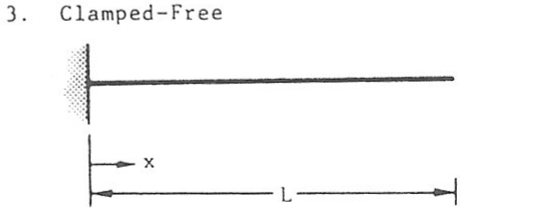
\includegraphics[width=0.4\textwidth]{blevins_beam.png}}}
\caption{Image of a cantilevered beam model.  From ``Formulas for Natural Frequency and Mode Shape'' by R. D. Blevins.}
\label{f:blevins}
\end{figure}
The resulting expression for the first natural frequency, in \unitfrac[]{rad}{s}, is
\begin{equation}\label{e:blevins}
\omega_n = \frac{(1.875)^2}{L^2} \sqrt{\left( \frac{EI}{\rho} \right)}
\end{equation}
where $\rho$ is the mass per unit length of the beam (the product of the density and the cross-section area), $E$ is the modulus of elasticity of the beam material, $I$ is the second moment of area of the beam and $L$ is the length of the beam. 

\subsection{First-Mode of Cantilevered Beam with Added Mass}
Similarly, it is possible to predict the natural frequency of a uniform cantilevered beam with a point-mass at the free end of the beam as illustrated in Figure~\ref{f:blevinsmass}.
\begin{figure}[htb!]
\centerline{
{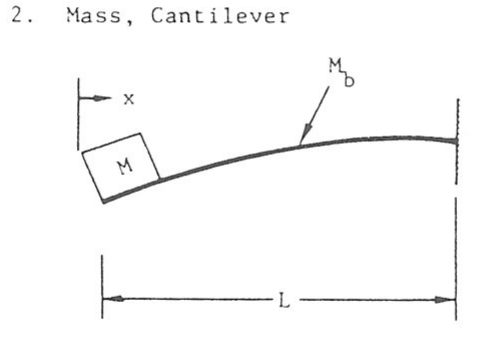
\includegraphics[width=0.4\textwidth]{blevins_beam_mass.png}}}
\caption{Image of a cantilevered beam with point mass model from ``Formulas for Natural Frequency and Mode Shape'' by R. D. Blevins.}
\label{f:blevinsmass}
\end{figure}
The first natural frequency for this model is
\begin{equation}\label{e:blevinsmass}
\omega_n = \sqrt{ \frac{3 E I}{L^3 (M+0.24 M_b)}}
\end{equation}
where $M$ is the point mass at the free end of the beam and $M_b$ is the total mass of the beam.

Notice that both predicted natural frequencies (\ref{e:blevins}) and (\ref{e:blevinsmass}) have the general from of $\omega_n = \sqrt{K/M}$ where $K$ is the ``stiffness'' of the system and $M$ is the ``mass'' of the system.


\begin{ex}\label{ex:beamvib}
Given a uniform cantilevered beam with the following properties:
\begin{itemize}
\item Length = \unit[0.5]{m}
\item Width = \unit[2.54]{cm}
\item Thickness = \unit[1.59]{mm}
\item Modulus of Elasticity ($E$) = \unit[68.9]{GPa}
\item Density = \unitfrac[2.70]{g}{cm$^3$}
\end{itemize}
Predict the undamped natural frequency.  Express the answer in both of the following units: \unitfrac[]{rad}{s} and \unit[]{Hz}.
\end{ex}

\ifsolutions
\begin{soln}
Use (\ref{e:blevins}) with the values from the Exercise.  The mass-per-unit-length is the product of the density and the cross-sectional area:
\[ \rho = D*(t*W) \]
where $D$ is the density, $t$ is the beam thickness and $W$ is the beam width.
We also need to calculate the second moment of area...
\[ I = 1/12(W*t^3) \]
If we plug in these values we get...
\[ \omega_n = \unitfrac[32.6]{rad}{s} \]
To express in Hz
\[ f_n = \frac{\unitfrac[\omega_n]{rad}{s}}{\unitfrac[2\pi]{rad}{cycle}} = \unitfrac[5.2]{cycles}{s}=\unit[5.2]{Hz}
\]

\lstinputlisting[style=myMatStyle,
caption={Script for predicting the natural frequency of a cantilevered beam.},
label={l:natlfreq}]
{../code/natl_freq_pred.m}

\end{soln}
\fi

\begin{ex}\label{ex:model2sim}
Given the uniform cantilevered beam described in the previous example, and a damping ratio of $\zeta=0.02$ (2\% damping)...
\begin{itemize}
\item Write an expression for a mathematical model of the form in (\ref{e:second}) to describe the system.  (You should just need to substitute in numerical values for the system parameters $\zeta$ and $\omega_n$.)
\item Using MATLAB, produce a graph that predicts the response of the tip of the cantilevered beam to an initial displacement of \unit[1.0]{cm} and zero initial velocity: $y(0)=\unit[1.0]{cm}$ and $\dot{y}(0) = \unitfrac[0]{cm}{s}$.
\end{itemize}
\end{ex}

\ifsolutions
\begin{soln}
\[
\ddot{y}(t) + 2 (0.02) (32.6)\dot{y}(t) + (32.6)^2 = f(t)
\]
To generate the graph we can use the same script from Exercise~\ref{ex:secondresp} and substitute in the new values for $\zeta$ and $\omega_n$.

\lstinputlisting[style=myMatStyle,
caption={Script for plotting the corrected free response of a second-order model using the given beam parameters.},
label={l:secondfreemodelsoln}]
{../code/second_order_free_model.m}

\begin{figure}[hbt]
\centering
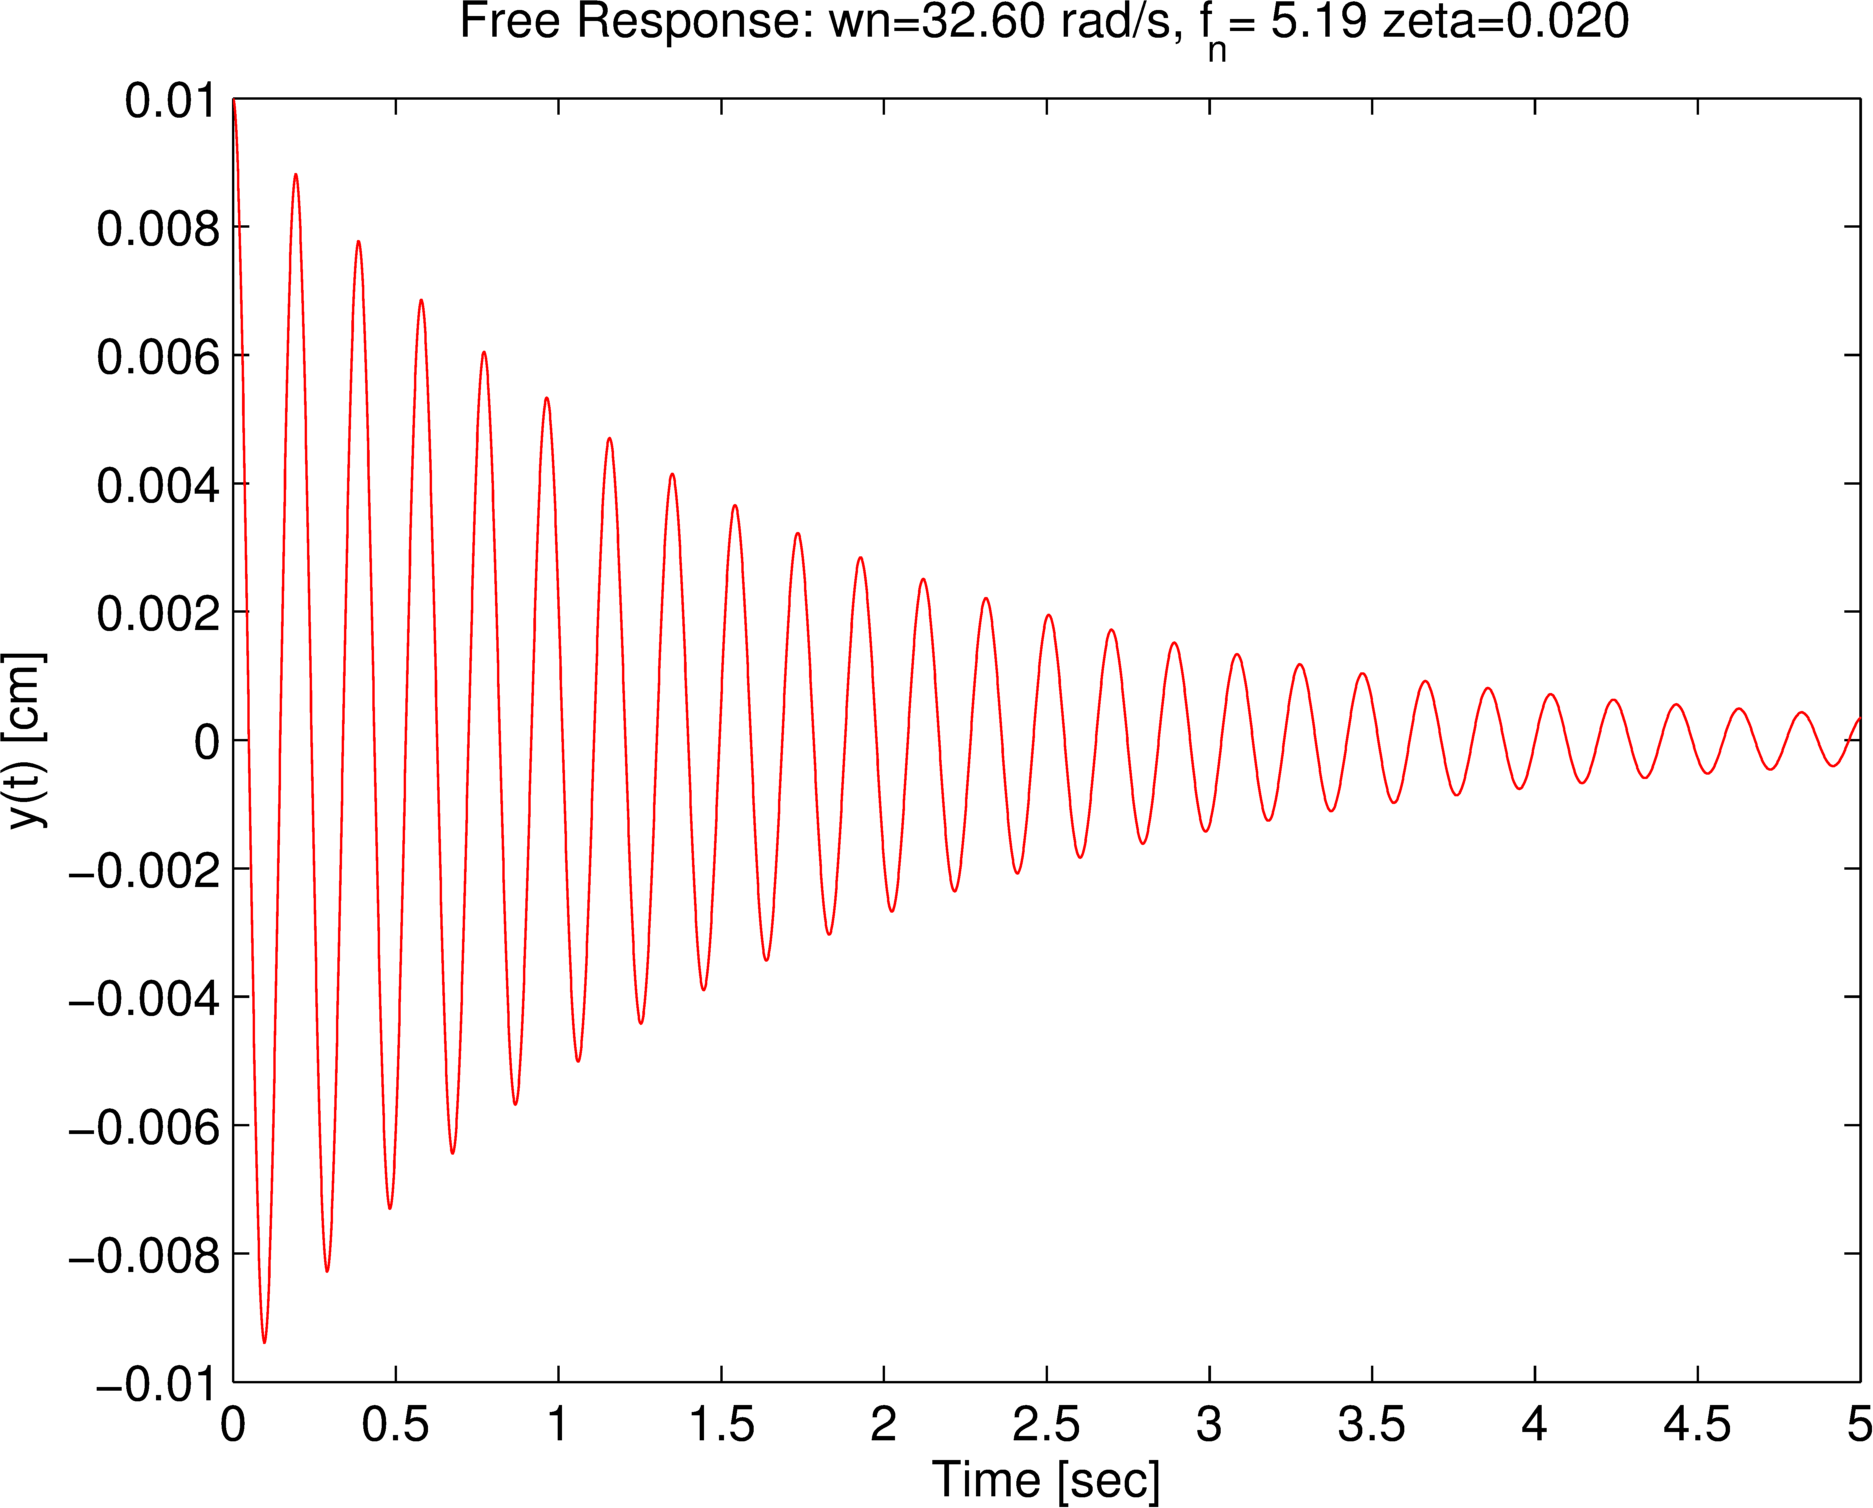
\includegraphics[width=\FigWidth\textwidth]{soln_second_free_model.png}
\caption{Graphs of the second-order free response for the predicted natural frequency from the given beam parameters.}
\label{f:soln2freemodel}
\end{figure}

\end{soln}
\fi


%\section{The Laplace Transform}

%\section{The Transfer Function}

\section{Numerical Solutions}
One reason that the first and second order models are a good place to start our discussion is that both of these differential equations have analytical (or closed-form) solutions, i.e., a solution that satisfies the differential equation can be expressed as a function.  This provides us instant gratification; we can (hopefully) clearly see how the parameters of the model (the mass, damping, etc.) affect the solution (how fast it changes, whether it oscillates, etc.).   Often the model we are interested in using doesn't have a tractable analytical solution.  Instead we need to rely on numerical approximations to predict the response of our model using computational tools.

\subsection{Solution for first-order ODE}
Numerical solutions to the differential equations based models common in robotics can be implemented using numerical integration.  A simple, but sometimes brittle, algorithm is Euler integration.  Consider a first-order differential equation $\dot{y}(t)=f(t,y(t))$.  If we integrate this expression for $\dot{y}(t)$ will will generate a solution model---$y(t)$.   To get things started we also need to no the initial condition of the function, where to start, which can be expressed as $y(t=0)=y_0$.  Euler integration is now a set of discrete, repeated steps to approximate the solution.  We can start at our initial time $t=0$ were we already know the answer
\[
y(t=0) = y_0.
\]
Now we step forward in time by some small increment in time $dt$ 
\begin{eqnarray}
y(dt) & = & y(0) + \left(\dot{y}(0)\right)(dt) \\
      & = & y_0 + (f(t=0,y(t=0)))(dt) \\
      & = & y_0 + (f(0,y_0))(dt).
\end{eqnarray}
Then we can step forward again by the same time increment
\begin{eqnarray}
y(2(dt)) & = & y(dt) + \left(\dot{y}(dt)\right)(dt) \\
         & = & \left(y_0 + (f(0,y_0))(dt)\right) + (f(dt,(y_0 + (f(0,y_0))(dt)))(dt).
\end{eqnarray}
As we continue to step forward we follow the same step: take the old value of $y(t)$, evaluate our expression for the derivative $\dot{y}$ at the previous time step and sum the previous value of $y(t)$ with the product of the derivative and step size $\dot{y}(t)(dt)$.  To express this efficiently we can break up continuous time into a set of discrete steps $t_k = t_0+k(dt)$.  The Euler method for solving this first-order ODE gives us an approximation for the solution at each of these discrete steps. This discrete values will be noted as $y[k] = y(t_k=t_0+k(dt)$ so we can now express the solution at discrete times as
\[
y[k+1] = y[k] + \dot{y}[k](dt) = y[k] + f(t_k,y[k])(dt).
\]
Now we have an algorithm that is well-suited for implementing with a computer program.  An illustrative example is given in Listing~\ref{l:firstorder_euler}.
\lstinputlisting[style=myMatStyle,
caption={Numerical solution for a first-order ODE using Euler integration: firstorder\_euler.m},
label={l:firstorder_euler}]
{../code/firstorder_euler.m}

\begin{ex}
Listing~\ref{l:carresp} illustrates how to graph the analytical solution to a first-order ODE model of a vehicle moving in one dimension.  Adapt Listing~\ref{l:firstorder_euler} to solve the same problem solved analytically in Listing~\ref{l:carresp}. 
\begin{itemize}
\item Create a graph that includes both the analytical solution and the numerical solution on the same axes.  You should use different line types (and/or symbols) along with a legend annotate the graph.
\item Create a second graph that displays the error between the two solutions ($y_{\mathrm{analytical}} - y_{\mathrm{numerical}}$) as a function of time.
\end{itemize}
\end{ex}

\begin{ex}
Start with the program in Listing~\ref{l:firstorder_euler} and increase the value of the timestep ($dt$).  
\begin{itemize}
\item What is the maximum value of $dt$ that successfully reproduces the first-order response that we expect?  Report the maximum value of $dt$ and the ratio of $dt/\tau$.  
\item Choose a value for $dt$ that is 1.8 times the size of the time constant.  Plot the numerical solution ($y(t)$) as a function of time.  Write a short explanation (a few sentences) to describe what you observe.
\item Repeat the above exercise with a value of $dt$ that is 2.5 times the size of the time constant.
\end{itemize}
\end{ex}

\ifsolutions


\begin{figure}[hbt]
\centering
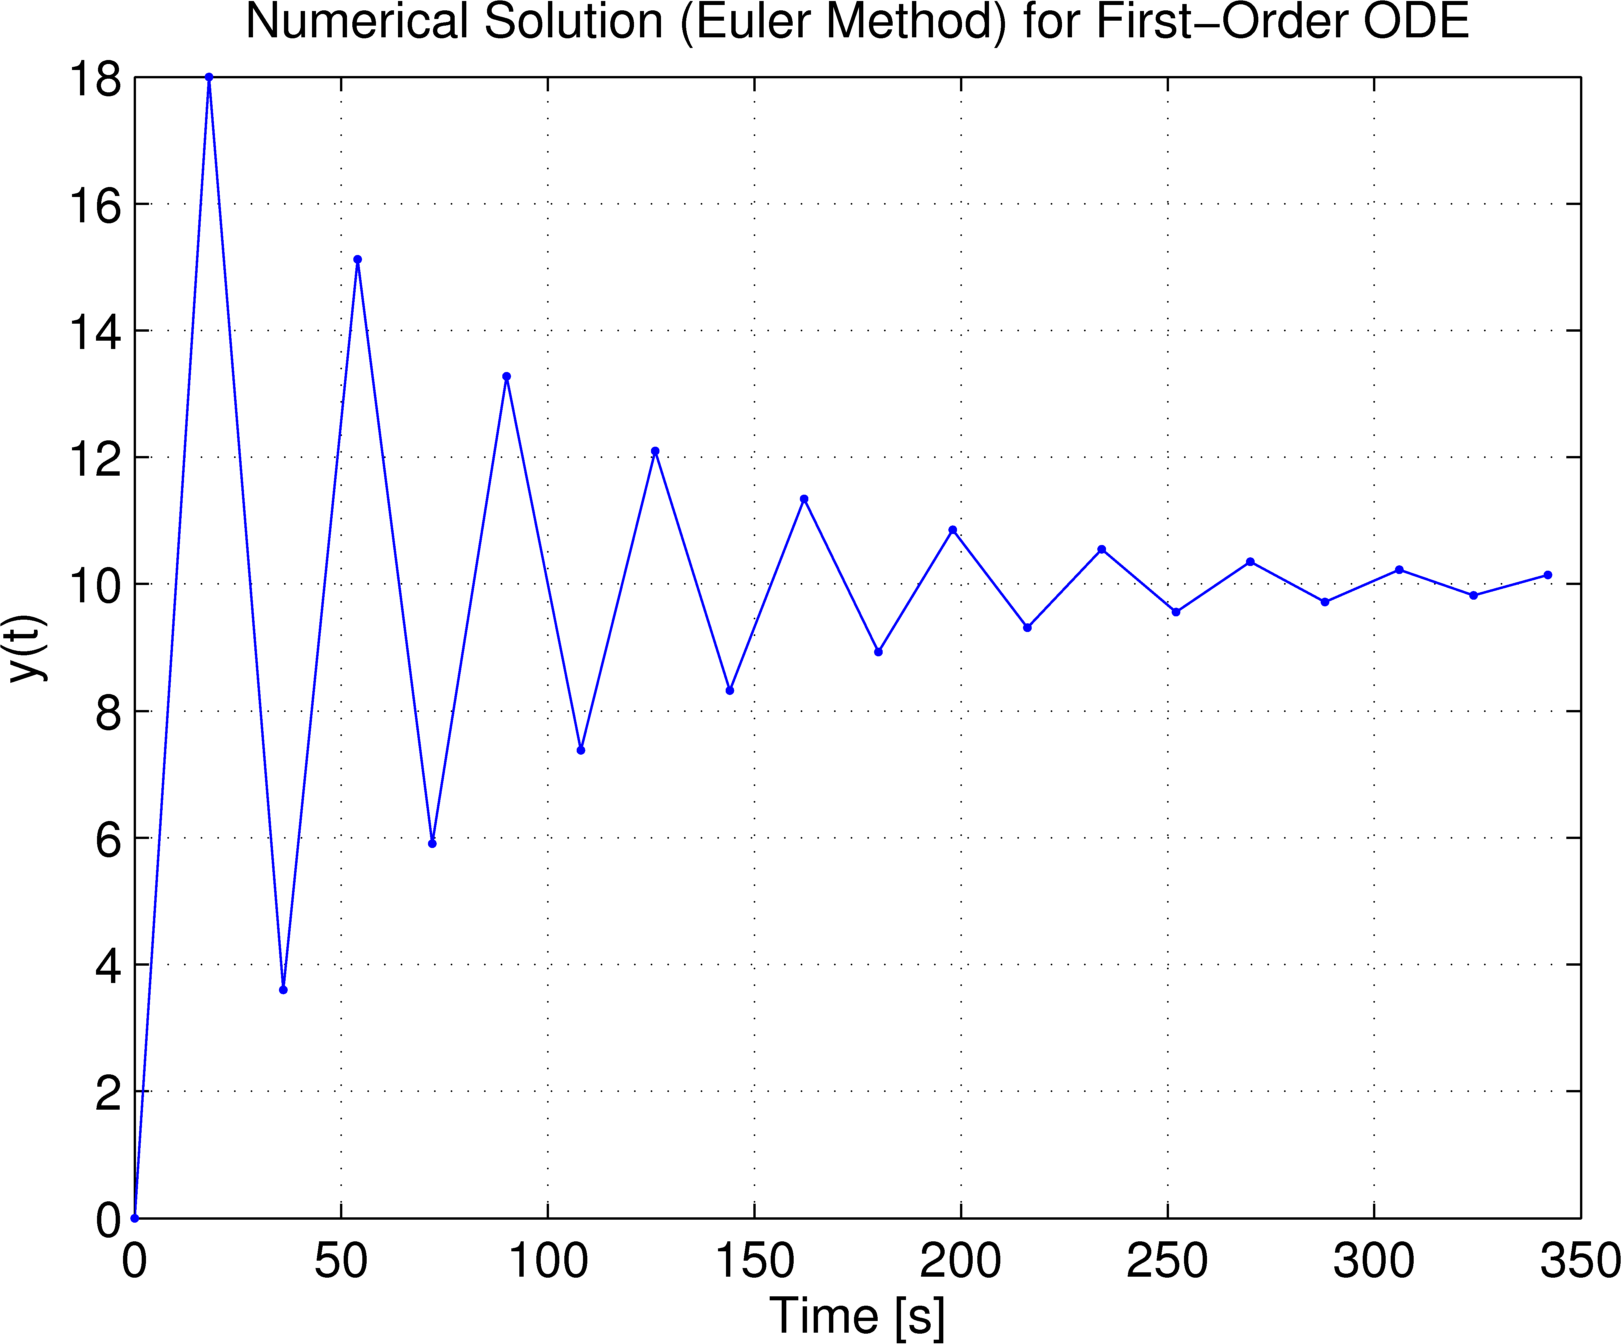
\includegraphics[width=\FigWidth\textwidth]{../code/firstorder_euler_soln.png}
\caption{dt = 1.8 times tau}
\label{f:euler_soln1}
\end{figure}

\begin{figure}[hbt]
\centering
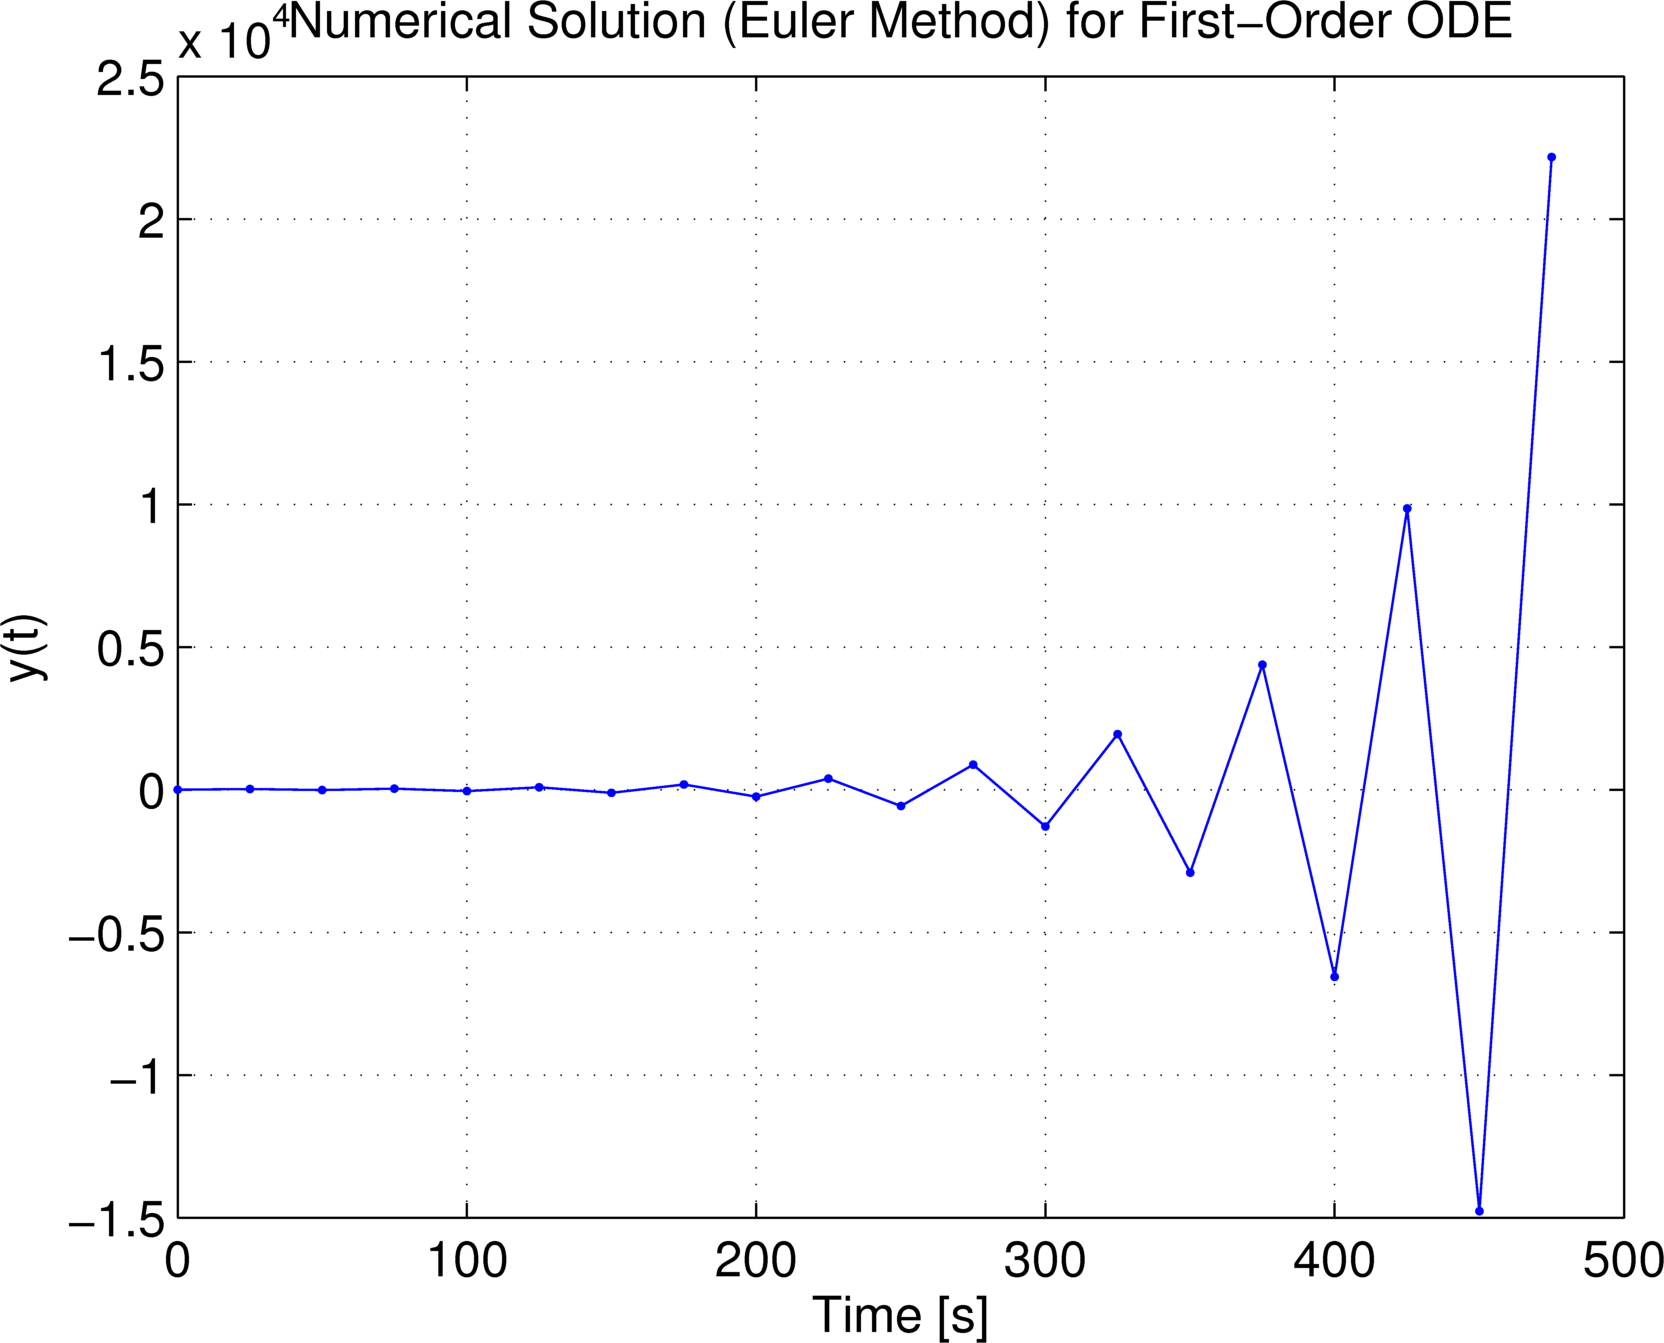
\includegraphics[width=\FigWidth\textwidth]{../code/firstorder_euler_soln2.png}
\caption{dt = 2.5 times tau}
\label{f:euler_soln2}
\end{figure}

\begin{soln}
\end{soln}
\fi


\subsection{Solution for higher-order ODEs}
We can extend this same approach to higher order models.  The key step in this extension is to transform the higher order ODE into a set of first-order ODEs.  (When we discuss linear algebra later in this text we'll see how this can be done efficiently.)  To start with an example we'll revisit our canonical second order model from (\ref{e:second}) repeated here:
\begin{equation} 
\ddot{y}(t) + 2 \zeta \omega_n (\dot{y}(t)) + \omega_n^2 (y(t)) = f(t).
\end{equation} 
To transform this second order ODE into two coupled first order ODEs we need to introduce two auxiliary variables which we might call the \emph{states} of the system:
\begin{eqnarray}
x_1(t) & = & y(t) \\
x_2(t) & = & \dot{y}(t).
\end{eqnarray}
Now we express the first derivative of these states using the second order model which yields
\begin{eqnarray}
\dot{x}_1(t) & = & \dot{y}(t) = x_2(t) \\
\dot{x}_2(t) & = & \ddot{y}(t) = -2 \zeta \omega_n x_2(t) - \omega_n^2 x_1(t) + f(t) 
\end{eqnarray}
Next we use the same Euler integration approach above to step forward in time, starting from the initial conditions: $y(t=0)=x_1(t=0)=y_0$ and $\dot{y}(t=0)=x_2(t=0)=\dot{y}_0$.  This results in computational algorithm
\begin{eqnarray}
x_1[k+1] & = & x_1[k] + x_2[k](dt) \\
x_2[k+1] & = & x_2[k] + \left(-2 \zeta \omega_n (x_2[k]) - \omega_n^2 (x_1[k]) + f[k]\right) (dt) 
\end{eqnarray}
where $f[k]$ is the forcing function (the input) at time $t=k(dt)$.

\begin{ex}
The analytical solution in (\ref{e:secondfree_annote} is the closed-form solution to our second order model.  Listing~\ref{l:secondfree} attempts to graph this solution given values for the model parameters and initial conditions.
\begin{itemize}
\item Develop a program to numerically approximate the solution of the model under these conditions and graph the solution $y(t)$ with respect to time.
\item To develop this program you will have to have chosen a time increment size, a timestep.  Starting from a working simulation, increase the size of this timestep until the solution is no longer stable.  Report the maximum allowable timestep value as the value of $dt$ and the ratio of $dt/\omega$.
\end{itemize}
\end{ex}








\printglossary[type=\thisgls]
\glsresetall

\renewcommand{\thisgls}{feedback}

\newglossaryentry{feedback}
{type=\thisgls,
name={linear system},
description={A linear system is a system which is linear.}
symbol={}
}

\chapter{Feedback}\label{c:feedback}
\section{Uses of Feedback}

disturbance rejection
parameter sensitivity
command tracking
\section{Anatomy of Feedback Control}

\begin{figure}[hbt]
\centering
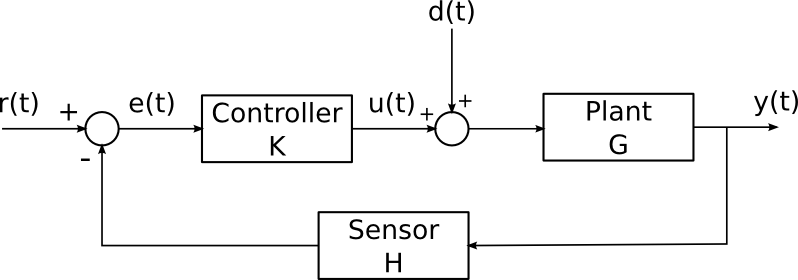
\includegraphics[width=\FigWidth\textwidth]{feedback.png}
\caption{Canonical feedback control system block diagram.}
\label{f:fdbk}
\end{figure}

process
disturbance
actuator
plant 
controller
sensor


\section{PID Control}

\section{Assessing Stability}

\section{Assessing Performance}

This chapter is about \gls{feedback}s.

\printglossary[type=\thisgls]
\glsresetall

\renewcommand{\thisgls}{models}

\newglossaryentry{robotmodel}
{type=\thisgls,
name={linear system},
description={A linear system is a system which is linear.}
symbol={}
}

\chapter{Robot Models}\label{c:models}
\section{Direct Drive Horizontal Model}

\begin{figure}[hbt]
\centering
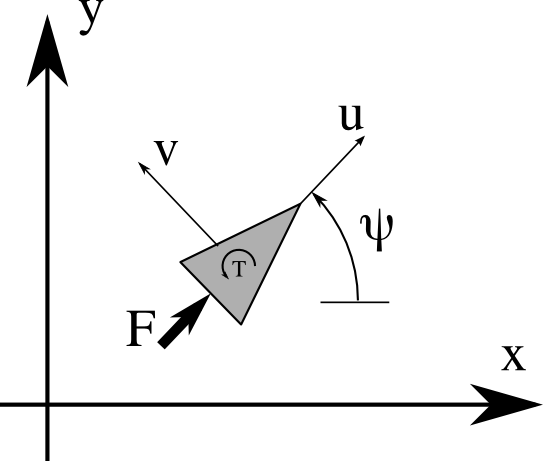
\includegraphics[width=\FigWidth\textwidth]{uni_model.png}
\caption{Illustration of the direct drive horizontal robot model.}
\label{f:uni_model}
\end{figure}

Three degrees of freedom.

\begin{itemize}
\item Model States
\begin{itemize}
\item $x$ and $y$: Position of the vehicle with respect to a fixed frame of reference.
\item $\psi$: Angular position of the vehicle relative to the $x$ axis.
\item $u$: Forward velocity of the vehicle with respect to the body-frame.
\item $v$: Lateral velocity of the vehicle with respect to the body-frame.
\item $r$: Angular velocity of the vehicle.
\end{itemize}
\item Inputs
\begin{itemize}
\item $F$: Force input in the foward direction with respect to the body-frame.
\item $T$: Torque input in the counter-clockwise direction.
\end{itemize}
\item Model Parameters
\begin{itemize}
\item $M$: Tranlational intertia (mass) of the vehicle
\item $I$: Rotational inertia (moment-of-inertia) of the vehicle
\item $d_u$: Tranlational damping/drag on the vehicle in the forward ($u$) direction
\item $d_v$: Tranlational damping/drag on the vehicle in the lateral ($v$) direction
\item $d_r$: 
\end{itemize}
\end{itemize}

Kinematics

\begin{eqnarray}
\dot{x} & = & \cos{(\psi)}u - \sin{(\psi)}v \\
\dot{y} & = & \sin{(\psi)}u + \cos{(\psi)}v \\
\dot{\psi} & = & r
\end{eqnarray}

Kinetics
\begin{eqnarray}
\dot{u} & = & -\frac{d_u}{M}u + \frac{1}{M}F \\
\dot{v} & = & -\frac{d_v}{M}v \\
\dot{r} & = & -\frac{d_r}{I}r + \frac{1}{I}T \\
\end{eqnarray}
If the damping factors ($d_u$, $d_v$ and $d_r$) are constants, this model represents linear drag behavior.
This chapter is about \gls{robotmodel}s.

\begin{ex}
Write a simulation - write the discrete-time formulation on paper first
\end{ex}

\begin{ex}
Test the simulation with some test inputs
\end{ex}

\begin{ex}
Choose a constant dt based on physical parameters
\end{ex}

\begin{ex}
Write the simulation using some linear algebra
\end{ex}

\
\begin{ex}
Write an open-loop  controller
Write a closed-loop controller
\end{ex}

\begin{ex}
Reformulate for differential drive
Figure~\ref{f:uni_model_diff}
\end{ex}

\begin{figure}[hbt]
\centering
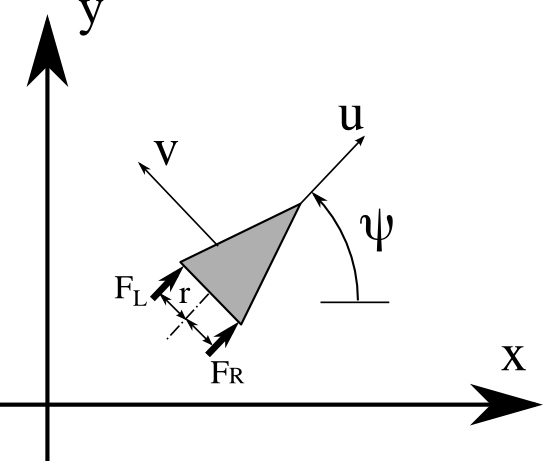
\includegraphics[width=\FigWidth\textwidth]{uni_model_diff.png}
\caption{Illustration of the differential drive variant of the horizontal robot model shown in Figure~\ref{f:uni_model}.}
\label{f:uni_model_diff}
\end{figure}

\printglossary[type=\thisgls]
\glsresetall

\renewcommand{\thisgls}{statespace}

\newglossaryentry{statespace}
{type=\thisgls,
name={linear system},
description={A linear system is a system which is linear.}
symbol={}
}

\chapter{State Space}\label{c:statespace}
\section{Introduction}
State-space is representation of dynamic models based on presenting the governing equations as a set of first-order differential equations.  This representation makes heavy use of linear algebra to compactly capture the set of differential equations.  By using this representation for the ODE-based models we can bring considerable mathematical tools to bear on the problem, giving us new methods to analyze the system, predict stability and performance and synthesize control algorithms.


\section{Canonical State-Space Form}
As the name implies, the state space representation is based on the state of the system, represented by a vector with $n$ elements. (The system is $n^{th}$ order.)  The representative form of a state space mathematical expression for a model with linear, time-invariant dynamics is a set of two matrix equations
\begin{align}\label{e:state-space}
\dot{\V{x}}(t) & = \V{A} \cdot \V{x}(t) + \V{B} \cdot \V{u}(t) \nonumber \\
\V{y}(t) & = \V{C} \cdot \V{x}(t) + \V{D} \cdot \V{u}(t)
\end{align}
where
\begin{itemize}
\item $\V{x}$(t) is the $n \times 1$ state vector,
\item $\V{A}$ is the $n \times n$ system matrix,
\item $\V{B}$ is the $n \times m$ input matrix,
\item $\V{u}$(t) is the $m \times 1$ input vector,
\item $\V{y}$(t) is the $p \times 1$ output vector,
\item $\V{C}$ is the $p \times n$ output matrix, and
\item $\V{D}$\footnote{Often the direct transmission term can be omitted because the input does not directly influence the output in the governing equations.} is the $p \times m$ direct transmission matrix\footnote{
Notation: We will try to be consistent with the following notation.  A vector variable is represented by a bold, lower-case variable, and when the elements of the vector shown curly brackets ($\mathbf{\{\}}$) are used.  A matrix variable is represented by a bold, upper-case variable, and when the elements of the matrix are shown square brackets ($\mathbf{[]}$) are used.  In (\ref{e:state-space}) the matrix products are highlighted by the dot-operator (e.g, $\V{A} \cdot \V{x}(t)$); for brevity this operator will not be included as we move forward.
}.
\end{itemize}
The first equation in (\ref{e:state-space}) captures the dynamics of the system---how the state changes with time and in response to a set of inputs $\V{u}$.  The second equation in (\ref{e:state-space}) describes how the outputs of the system $\V{y}$ (typically the quantities we can observe or measure) are related to the internal states of the system and perhaps the input.




The continuous-time dynamics of the mathematical model are described in (\ref{e:state-space}).  A discrete time approximation can be written in a similar form
\begin{align}
\label{e:state-spaced}
\V{x}[k+1] & = \V{F} \V{x}[k] + \V{G}\V{u}[k] \nonumber \\
\V{y}[k] & = \V{H}\V{x}[k] + \V{J}\V{u}[k]
\end{align}
where
\begin{itemize}
\item $\V{x}[k]$ is the $n \times 1$ state vector at time $t=k(dt)$,
\item $\V{G}$ is the $n \times n$ system matrix,
\item $\V{F}$ is the $n \times m$ input matrix,
\item $\V{u}[k]$ is the $m \times 1$ input vector at time $t=k(dt)$,
\item $\V{y}[k]$ is the $p \times 1$ output vector at time $t=k(dt)$,
\item $\V{H}$ is the $p \times n$ output matrix, and
\item $\V{J}$ is the $p \times m$ direct transmission matrix.
\end{itemize}

\subsection{Example: Second-Order System}
Recall in Section~\ref{ss:higher-order} that we transformed our second-order model 
\begin{equation}\label{e:2ndagain}
\ddot{y}(t) + 2 \zeta \omega_n (\dot{y}(t)) + \omega_n^2 (y(t)) = f(t)
\end{equation}
into two coupled first-order ODEs by defining two states of the system
\begin{align}\label{e:2states}
x_1(t) & = y(t) \nonumber \\
x_2(t) & = \dot{y}(t).
\end{align}
We can now write this model in our canonical state space form with the state vector
\[
\V{x}(t)  =  \left\{ \begin{array}{c}
x_1(t) \\
x_2(t) 
\end{array} \right\}
\]
as 
\begin{align}\label{e:state-space-2d}
\dot{\V{x}}(t) & = \left[ \begin{array}{cc}
0 & 1 \\
-\omega_n^2 & -2 \zeta \omega_n  
\end{array} \right] \V{x}(t) + 
\left[ \begin{array}{c}
0 \\
1
\end{array}\right]
f(t) \nonumber \\
y(t) & = \left[ \begin{array}{cc} 1 & 0 \end{array} \right] \V{x}(t)
\end{align}

\begin{ex}
Write a new state space description of the model (\ref{e:2ndagain}) with the state definition
\[
\V{x}(t)  =  \left\{ \begin{array}{c}
\dot{y}(t) \\
y(t)
\end{array} \right\}.
\]
As shown in the example, the input to the system is the scalar $f(t)$ and the output of the system is the scalar $y(t)$. 
\end{ex}

\begin{ex}
Write the discrete approximation of our second-order ODE given in (\ref{e:2nd-euler} in the discrete state-space form (\ref{e:state-spaced}.  Note that $\V{F}$ and $\V{G}$ will be functions of the time-step $dt$.
\end{ex}


\section{Numerical Approximation}
Once we have out model dynamics expressed in state space form (\ref{e:state-space}) there are a variety of ways of approximating the solution to this set of ODEs using numerical integration.  Perhaps the simplest (but not terribly accurate) method is to apply the forward Euler method discussed in Section~\ref{s:numerical}, expanding the approach from scalar-valued ODEs to vector-valued ODEs.  Using this technique we can approximate the state at time $k+1$ using the previous state, the rate-of-change of the state given by (\ref{e:state-space}) and the constant scalar value for the time-step ($\dt$) as
\begin{align}
\label{e:state-space-euler}
\V{x}[k+1] & = \V{x}[k] + \dot{\V{x}}[k](\dt) \nonumber \\
           & = \V{x}[k] + \left[\V{A}\V{x}[k]+\V{B}\V{u}[k]\right](\dt) \nonumber \\
           & = \left[\V{I}+\V{A}(\dt)\right]\V{x}[k] + \left[\V{B}(\dt)\right]\V{u}[k]. \nonumber \\
\V{y}[k+1] & = \V{C}\V{x}[k+1] + \V{D}\V{u}[k]
\end{align}
So using Euler integration our numerical approximation (\ref{e:state-spaced}) of the continuous time state space model is
\begin{align}
\label{e:state-space-euler2}
\V{F} & = \left[\V{I}+\V{A}(\dt)\right] \nonumber \\
\V{G} & = \left[\V{B}(\dt)\right] \nonumber \\
\V{H} & = \V{C} \nonumber \\
\V{J} & = \V{D}
\end{align}

\section{Exercises}
\begin{ex}
Write the equations of motion for our direct drive horizontal model ((\ref{e:direct_kinematics}) and (\ref{e:direct_kinetics})) in the canonical state space form (\ref{e:state-space}).  This system is non-linear so the matrices will be non-linear functions of some of the state variables.
\end{ex}

\begin{ex}
Create a computational simulation of the model (i.e, a numerical approximation of the solution to the system of ODEs) using the parameters given in Exercise~\ref{ex:direct_sim}.  Formulate your numerical approximation using the continuous-time dynamics (in state space form) and the forward Euler approximation (\ref{e:state-space-euler}).  This computational solution should make use of matrix operations (multiplication). 

Illustrate that your simulation behaves the same as your scalar implementation from Exercise~\ref{ex:direct_sim}.
\end{ex}

\section{Control Exercises}

\begin{ex}
In this exercise you will develop a cruise control algorithm for the direct drive robot model in (\ref{e:direct_kinematics}) and (\ref{e:direct_kinetics}).  Use the parameters in given in Exercise~\ref{ex:direct_sim} for the model.  In addition our robot has limited actuation authority; it can supply a maximum of \unit[10]{N} of thrust and \unit[10]{N$\cdot$m} of torque.  Your controllers should attempt to minimize rise-time, overshoot and steady-state error while observing these maximums.

Start by working on a heading controller.  Develop a control algorithm that takes a heading setpoint and calculates a torque to achieve the setpoint.  You can test the response of this algorithm using step inputs.  A reasonable size of the step input is $\pi/2$ radians.  To deal with any quadrant errors it is recommended that you verify your heading controller works for the following scenarios:
\begin{itemize}
\item Initial Heading: \unit[0]{rad}, Heading Goal: \unit[$pi/2$]{rad}
\item Initial Heading: \unit[0]{rad}, Heading Goal: \unit[-$pi/2$]{rad}
\item Initial Heading: \unit[$3\pi/4$]{rad}, Heading Goal: \unit[$5pi/4$]{rad}
\item Initial Heading: \unit[$5\pi/4$]{rad}, Heading Goal: \unit[$3pi/4$]{rad}
\end{itemize}
This assumes all other states have zero initial conditions.

Now put that aside and work on a velocity controller (with no heading control).  Develop a control algorithm that takes a velocity setpoint and calculates a forward thrust to achieve the setpoint.  Test your controller with the following scenarios:
\begin{itemize}
\item Initial Heading: \unit[0]{rad}, Initial Forward Velocity: \unitfrac[0]{m}{s}, Velocity Goal: \unitfrac[1.0]{m}{s}
\item Initial Heading: \unit[0]{rad}, Initial Forward Velocity: \unitfrac[1.0]{m}{s}, Velocity Goal: \unitfrac[0]{m}{s}
\end{itemize}

Now we are ready to put these two independent controllers together into a \emph{hybrid} controller to regulate both heading and velocity.  Demonstrate the behavior of your controller with the following sequential commands:
\begin{enumerate}
\item Begin with zero initial conditions on all states
\item Provide your controller with a heading goal of \unit[$\pi/4$]{rad} and a velocity goal of \unitfrac[0.5]{m}{s} for \unit[5]{s}.
\item Provide your controller with a heading goal of \unit[$3\pi/4$]{rad} and a velocity goal of \unitfrac[1.0]{m}{s} for \unit[5]{s}.
\end{enumerate}

Submit the following:
\begin{itemize}
\item A short description of your heading and velocity controllers - what are your controllers doing?
\item A graph of the x-y position of reported by your model for the final scenario.
\item Graphs of the states of your model as a function of time for the final scenario.
\item A discussion of what is pertinent in the graphs - what do you observe that makes you think the simulation and controllers are acting appropriately?
\end{itemize}
\end{ex}






\printglossary[type=\thisgls]
\glsresetall

%% Bibiliography
%\bibliographystyle{../latexlib/latex_ieee/IEEEtran}
%\bibliography{../bibtex/ref_bbing_master}


% that's all folks
% that's all folks
\end{document}


